\documentclass[12pt,a4paper,]{book}
\def\ifdoblecara{} %% set to true
\def\ifprincipal{} %% set to true
\let\ifprincipal\undefined %% set to false
\def\ifcitapandoc{} %% set to true
\let\ifcitapandoc\undefined %% set to false
\usepackage{lmodern}
\usepackage{amssymb,amsmath}
\usepackage{ifxetex,ifluatex}
%\usepackage{fixltx2e} % provides \textsubscript %PLLC
\ifnum 0\ifxetex 1\fi\ifluatex 1\fi=0 % if pdftex
  \usepackage[T1]{fontenc}
  \usepackage[utf8]{inputenc}
\else % if luatex or xelatex
  \ifxetex
    \usepackage{mathspec}
  \else
    \usepackage{fontspec}
  \fi
  \defaultfontfeatures{Ligatures=TeX,Scale=MatchLowercase}
\fi
% use upquote if available, for straight quotes in verbatim environments
\IfFileExists{upquote.sty}{\usepackage{upquote}}{}
% use microtype if available
\IfFileExists{microtype.sty}{%
\usepackage{microtype}
\UseMicrotypeSet[protrusion]{basicmath} % disable protrusion for tt fonts
}{}
\usepackage[margin = 2.5cm]{geometry}
\usepackage{hyperref}
\hypersetup{unicode=true,
            pdfauthor={Gloria Vizcaíno Castaño},
              pdfborder={0 0 0},
              breaklinks=true}
\urlstyle{same}  % don't use monospace font for urls
\usepackage{natbib}
\bibliographystyle{plainnat}
\usepackage[usenames,dvipsnames]{xcolor}  %new PLLC
\usepackage{longtable,booktabs}
\IfFileExists{parskip.sty}{%
\usepackage{parskip}
}{% else
\setlength{\parindent}{0pt}
\setlength{\parskip}{6pt plus 2pt minus 1pt}
}
\setlength{\emergencystretch}{3em}  % prevent overfull lines
\providecommand{\tightlist}{%
  \setlength{\itemsep}{0pt}\setlength{\parskip}{0pt}}
\setcounter{secnumdepth}{5}
% Redefines (sub)paragraphs to behave more like sections
\ifx\paragraph\undefined\else
\let\oldparagraph\paragraph
\renewcommand{\paragraph}[1]{\oldparagraph{#1}\mbox{}}
\fi
\ifx\subparagraph\undefined\else
\let\oldsubparagraph\subparagraph
\renewcommand{\subparagraph}[1]{\oldsubparagraph{#1}\mbox{}}
\fi

%%% Use protect on footnotes to avoid problems with footnotes in titles
\let\rmarkdownfootnote\footnote%
\def\footnote{\protect\rmarkdownfootnote}


  \title{}
    \author{Gloria Vizcaíno Castaño}
      \date{27/10/2017}


%%%%%%% inicio: latex_preambulo.tex PLLC

%% UTILIZA CODIFICACIÓN UTF-8
%% MODIFICARLO CONVENIENTEMENTE PARA USARLO CON OTRAS CODIFICACIONES


%\usepackage[spanish,es-nodecimaldot,es-noshorthands]{babel}
\usepackage[spanish,es-nodecimaldot,es-noshorthands,es-tabla]{babel}
% Ver: es-tabla (en: https://osl.ugr.es/CTAN/macros/latex/contrib/babel-contrib/spanish/spanish.pdf)
% es-tabla (en: https://tex.stackexchange.com/questions/80443/change-the-word-table-in-table-captions)
\usepackage{float}
\usepackage{placeins}
\usepackage{fancyhdr}
% Solucion: ! LaTeX Error: Command \counterwithout already defined.
% https://tex.stackexchange.com/questions/425600/latex-error-command-counterwithout-already-defined
\let\counterwithout\relax
\let\counterwithin\relax
\usepackage{chngcntr}
%\usepackage{microtype}  %antes en template PLLC
\usepackage[utf8]{inputenc}
\usepackage[T1]{fontenc} % Usa codificación 8-bit que tiene 256 glyphs

%\usepackage[dvipsnames]{xcolor}
%\usepackage[usenames,dvipsnames]{xcolor}  %new
\usepackage{pdfpages}
%\usepackage{natbib}




% Para portada: latex_paginatitulo_mod_ST02.tex (inicio)
\usepackage{tikz}
\usepackage{epigraph}
\input{portadas/latex_paginatitulo_mod_ST02_add.sty}
% Para portada: latex_paginatitulo_mod_ST02.tex (fin)

% Para portada: latex_paginatitulo_mod_OV01.tex (inicio)
\usepackage{cpimod}
% Para portada: latex_paginatitulo_mod_OV01.tex (fin)

% Para portada: latex_paginatitulo_mod_OV03.tex (inicio)
\usepackage{KTHEEtitlepage}
% Para portada: latex_paginatitulo_mod_OV03.tex (fin)

\renewcommand{\contentsname}{Índice}
\renewcommand{\listfigurename}{Índice de figuras}
\renewcommand{\listtablename}{Índice de tablas}
\newcommand{\bcols}{}
\newcommand{\ecols}{}
\newcommand{\bcol}[1]{\begin{minipage}{#1\linewidth}}
\newcommand{\ecol}{\end{minipage}}
\newcommand{\balertblock}[1]{\begin{alertblock}{#1}}
\newcommand{\ealertblock}{\end{alertblock}}
\newcommand{\bitemize}{\begin{itemize}}
\newcommand{\eitemize}{\end{itemize}}
\newcommand{\benumerate}{\begin{enumerate}}
\newcommand{\eenumerate}{\end{enumerate}}
\newcommand{\saltopagina}{\newpage}
\newcommand{\bcenter}{\begin{center}}
\newcommand{\ecenter}{\end{center}}
\newcommand{\beproof}{\begin{proof}} %new
\newcommand{\eeproof}{\end{proof}} %new
%De: https://texblog.org/2007/11/07/headerfooter-in-latex-with-fancyhdr/
% \fancyhead
% E: Even page
% O: Odd page
% L: Left field
% C: Center field
% R: Right field
% H: Header
% F: Footer
%\fancyhead[CO,CE]{Resultados}

%OPCION 1
% \fancyhead[LE,RO]{\slshape \rightmark}
% \fancyhead[LO,RE]{\slshape \leftmark}
% \fancyfoot[C]{\thepage}
% \renewcommand{\headrulewidth}{0.4pt}
% \renewcommand{\footrulewidth}{0pt}

%OPCION 2
% \fancyhead[LE,RO]{\slshape \rightmark}
% \fancyfoot[LO,RE]{\slshape \leftmark}
% \fancyfoot[LE,RO]{\thepage}
% \renewcommand{\headrulewidth}{0.4pt}
% \renewcommand{\footrulewidth}{0.4pt}
%%%%%%%%%%
\usepackage{calc,amsfonts}
% Elimina la cabecera de páginas impares vacías al finalizar los capítulos
\usepackage{emptypage}
\makeatletter

%\definecolor{ocre}{RGB}{25,25,243} % Define el color azul (naranja) usado para resaltar algunas salidas
\definecolor{ocre}{RGB}{0,0,0} % Define el color a negro (aparece en los teoremas

%\usepackage{calc} 

\usepackage{lipsum}

%\usepackage{tikz} % Requerido para dibujar formas personalizadas

%\usepackage{amsmath,amsthm,amssymb,amsfonts}
\usepackage{amsthm}


% Boxed/framed environments
\newtheoremstyle{ocrenumbox}% % Theorem style name
{0pt}% Space above
{0pt}% Space below
{\normalfont}% % Body font
{}% Indent amount
{\small\bf\sffamily\color{ocre}}% % Theorem head font
{\;}% Punctuation after theorem head
{0.25em}% Space after theorem head
{\small\sffamily\color{ocre}\thmname{#1}\nobreakspace\thmnumber{\@ifnotempty{#1}{}\@upn{#2}}% Theorem text (e.g. Theorem 2.1)
\thmnote{\nobreakspace\the\thm@notefont\sffamily\bfseries\color{black}---\nobreakspace#3.}} % Optional theorem note
\renewcommand{\qedsymbol}{$\blacksquare$}% Optional qed square

\newtheoremstyle{blacknumex}% Theorem style name
{5pt}% Space above
{5pt}% Space below
{\normalfont}% Body font
{} % Indent amount
{\small\bf\sffamily}% Theorem head font
{\;}% Punctuation after theorem head
{0.25em}% Space after theorem head
{\small\sffamily{\tiny\ensuremath{\blacksquare}}\nobreakspace\thmname{#1}\nobreakspace\thmnumber{\@ifnotempty{#1}{}\@upn{#2}}% Theorem text (e.g. Theorem 2.1)
\thmnote{\nobreakspace\the\thm@notefont\sffamily\bfseries---\nobreakspace#3.}}% Optional theorem note

\newtheoremstyle{blacknumbox} % Theorem style name
{0pt}% Space above
{0pt}% Space below
{\normalfont}% Body font
{}% Indent amount
{\small\bf\sffamily}% Theorem head font
{\;}% Punctuation after theorem head
{0.25em}% Space after theorem head
{\small\sffamily\thmname{#1}\nobreakspace\thmnumber{\@ifnotempty{#1}{}\@upn{#2}}% Theorem text (e.g. Theorem 2.1)
\thmnote{\nobreakspace\the\thm@notefont\sffamily\bfseries---\nobreakspace#3.}}% Optional theorem note

% Non-boxed/non-framed environments
\newtheoremstyle{ocrenum}% % Theorem style name
{5pt}% Space above
{5pt}% Space below
{\normalfont}% % Body font
{}% Indent amount
{\small\bf\sffamily\color{ocre}}% % Theorem head font
{\;}% Punctuation after theorem head
{0.25em}% Space after theorem head
{\small\sffamily\color{ocre}\thmname{#1}\nobreakspace\thmnumber{\@ifnotempty{#1}{}\@upn{#2}}% Theorem text (e.g. Theorem 2.1)
\thmnote{\nobreakspace\the\thm@notefont\sffamily\bfseries\color{black}---\nobreakspace#3.}} % Optional theorem note
\renewcommand{\qedsymbol}{$\blacksquare$}% Optional qed square
\makeatother



% Define el estilo texto theorem para cada tipo definido anteriormente
\newcounter{dummy} 
\numberwithin{dummy}{section}
\theoremstyle{ocrenumbox}
\newtheorem{theoremeT}[dummy]{Teorema}  % (Pedro: Theorem)
\newtheorem{problem}{Problema}[chapter]  % (Pedro: Problem)
\newtheorem{exerciseT}{Ejercicio}[chapter] % (Pedro: Exercise)
\theoremstyle{blacknumex}
\newtheorem{exampleT}{Ejemplo}[chapter] % (Pedro: Example)
\theoremstyle{blacknumbox}
\newtheorem{vocabulary}{Vocabulario}[chapter]  % (Pedro: Vocabulary)
\newtheorem{definitionT}{Definición}[section]  % (Pedro: Definition)
\newtheorem{corollaryT}[dummy]{Corolario}  % (Pedro: Corollary)
\theoremstyle{ocrenum}
\newtheorem{proposition}[dummy]{Proposición} % (Pedro: Proposition)


\usepackage[framemethod=default]{mdframed}



\newcommand{\intoo}[2]{\mathopen{]}#1\,;#2\mathclose{[}}
\newcommand{\ud}{\mathop{\mathrm{{}d}}\mathopen{}}
\newcommand{\intff}[2]{\mathopen{[}#1\,;#2\mathclose{]}}
\newtheorem{notation}{Notation}[chapter]


\mdfdefinestyle{exampledefault}{%
rightline=true,innerleftmargin=10,innerrightmargin=10,
frametitlerule=true,frametitlerulecolor=green,
frametitlebackgroundcolor=yellow,
frametitlerulewidth=2pt}


% Theorem box
\newmdenv[skipabove=7pt,
skipbelow=7pt,
backgroundcolor=black!5,
linecolor=ocre,
innerleftmargin=5pt,
innerrightmargin=5pt,
innertopmargin=10pt,%5pt
leftmargin=0cm,
rightmargin=0cm,
innerbottommargin=5pt]{tBox}

% Exercise box	  
\newmdenv[skipabove=7pt,
skipbelow=7pt,
rightline=false,
leftline=true,
topline=false,
bottomline=false,
backgroundcolor=ocre!10,
linecolor=ocre,
innerleftmargin=5pt,
innerrightmargin=5pt,
innertopmargin=10pt,%5pt
innerbottommargin=5pt,
leftmargin=0cm,
rightmargin=0cm,
linewidth=4pt]{eBox}	

% Definition box
\newmdenv[skipabove=7pt,
skipbelow=7pt,
rightline=false,
leftline=true,
topline=false,
bottomline=false,
linecolor=ocre,
innerleftmargin=5pt,
innerrightmargin=5pt,
innertopmargin=10pt,%0pt
leftmargin=0cm,
rightmargin=0cm,
linewidth=4pt,
innerbottommargin=0pt]{dBox}	

% Corollary box
\newmdenv[skipabove=7pt,
skipbelow=7pt,
rightline=false,
leftline=true,
topline=false,
bottomline=false,
linecolor=gray,
backgroundcolor=black!5,
innerleftmargin=5pt,
innerrightmargin=5pt,
innertopmargin=10pt,%5pt
leftmargin=0cm,
rightmargin=0cm,
linewidth=4pt,
innerbottommargin=5pt]{cBox}

% Crea un entorno para cada tipo de theorem y le asigna un estilo 
% con ayuda de las cajas coloreadas anteriores
\newenvironment{theorem}{\begin{tBox}\begin{theoremeT}}{\end{theoremeT}\end{tBox}}
\newenvironment{exercise}{\begin{eBox}\begin{exerciseT}}{\hfill{\color{ocre}\tiny\ensuremath{\blacksquare}}\end{exerciseT}\end{eBox}}				  
\newenvironment{definition}{\begin{dBox}\begin{definitionT}}{\end{definitionT}\end{dBox}}	
\newenvironment{example}{\begin{exampleT}}{\hfill{\tiny\ensuremath{\blacksquare}}\end{exampleT}}		
\newenvironment{corollary}{\begin{cBox}\begin{corollaryT}}{\end{corollaryT}\end{cBox}}	

%	ENVIRONMENT remark
\newenvironment{remark}{\par\vspace{10pt}\small 
% Espacio blanco vertical sobre la nota y tamaño de fuente menor
\begin{list}{}{
\leftmargin=35pt % Indentación sobre la izquierda
\rightmargin=25pt}\item\ignorespaces % Indentación sobre la derecha
\makebox[-2.5pt]{\begin{tikzpicture}[overlay]
\node[draw=ocre!60,line width=1pt,circle,fill=ocre!25,font=\sffamily\bfseries,inner sep=2pt,outer sep=0pt] at (-15pt,0pt){\textcolor{ocre}{N}}; \end{tikzpicture}} % R naranja en un círculo (Pedro)
\advance\baselineskip -1pt}{\end{list}\vskip5pt} 
% Espaciado de línea más estrecho y espacio en blanco después del comentario


\newenvironment{solutionExe}{\par\vspace{10pt}\small 
\begin{list}{}{
\leftmargin=35pt 
\rightmargin=25pt}\item\ignorespaces 
\makebox[-2.5pt]{\begin{tikzpicture}[overlay]
\node[draw=ocre!60,line width=1pt,circle,fill=ocre!25,font=\sffamily\bfseries,inner sep=2pt,outer sep=0pt] at (-15pt,0pt){\textcolor{ocre}{S}}; \end{tikzpicture}} 
\advance\baselineskip -1pt}{\end{list}\vskip5pt} 

\newenvironment{solutionExa}{\par\vspace{10pt}\small 
\begin{list}{}{
\leftmargin=35pt 
\rightmargin=25pt}\item\ignorespaces 
\makebox[-2.5pt]{\begin{tikzpicture}[overlay]
\node[draw=ocre!60,line width=1pt,circle,fill=ocre!55,font=\sffamily\bfseries,inner sep=2pt,outer sep=0pt] at (-15pt,0pt){\textcolor{ocre}{S}}; \end{tikzpicture}} 
\advance\baselineskip -1pt}{\end{list}\vskip5pt} 

\usepackage{tcolorbox}

\usetikzlibrary{trees}

\theoremstyle{ocrenum}
\newtheorem{solutionT}[dummy]{Solución}  % (Pedro: Corollary)
\newenvironment{solution}{\begin{cBox}\begin{solutionT}}{\end{solutionT}\end{cBox}}	


\newcommand{\tcolorboxsolucion}[2]{%
\begin{tcolorbox}[colback=green!5!white,colframe=green!75!black,title=#1] 
 #2
 %\tcblower  % pone una línea discontinua
\end{tcolorbox}
}% final definición comando

\newtcbox{\mybox}[1][green]{on line,
arc=0pt,outer arc=0pt,colback=#1!10!white,colframe=#1!50!black, boxsep=0pt,left=1pt,right=1pt,top=2pt,bottom=2pt, boxrule=0pt,bottomrule=1pt,toprule=1pt}



\mdfdefinestyle{exampledefault}{%
rightline=true,innerleftmargin=10,innerrightmargin=10,
frametitlerule=true,frametitlerulecolor=green,
frametitlebackgroundcolor=yellow,
frametitlerulewidth=2pt}





\newcommand{\betheorem}{\begin{theorem}}
\newcommand{\eetheorem}{\end{theorem}}
\newcommand{\bedefinition}{\begin{definition}}
\newcommand{\eedefinition}{\end{definition}}

\newcommand{\beremark}{\begin{remark}}
\newcommand{\eeremark}{\end{remark}}
\newcommand{\beexercise}{\begin{exercise}}
\newcommand{\eeexercise}{\end{exercise}}
\newcommand{\beexample}{\begin{example}}
\newcommand{\eeexample}{\end{example}}
\newcommand{\becorollary}{\begin{corollary}}
\newcommand{\eecorollary}{\end{corollary}}


\newcommand{\besolutionExe}{\begin{solutionExe}}
\newcommand{\eesolutionExe}{\end{solutionExe}}
\newcommand{\besolutionExa}{\begin{solutionExa}}
\newcommand{\eesolutionExa}{\end{solutionExa}}


%%%%%%%%


% Caja Salida Markdown
\newmdenv[skipabove=7pt,
skipbelow=7pt,
rightline=false,
leftline=true,
topline=false,
bottomline=false,
backgroundcolor=GreenYellow!10,
linecolor=GreenYellow!80,
innerleftmargin=5pt,
innerrightmargin=5pt,
innertopmargin=10pt,%5pt
innerbottommargin=5pt,
leftmargin=0cm,
rightmargin=0cm,
linewidth=4pt]{mBox}	

%% RMarkdown
\newenvironment{markdownsal}{\begin{mBox}}{\end{mBox}}	

\newcommand{\bmarkdownsal}{\begin{markdownsal}}
\newcommand{\emarkdownsal}{\end{markdownsal}}


\usepackage{array}
\usepackage{multirow}
\usepackage{wrapfig}
\usepackage{colortbl}
\usepackage{pdflscape}
\usepackage{tabu}
\usepackage{threeparttable}
\usepackage{subfig} %new
%\usepackage{booktabs,dcolumn,rotating,thumbpdf,longtable}
\usepackage{dcolumn,rotating}  %new
\usepackage[graphicx]{realboxes} %new de: https://stackoverflow.com/questions/51633434/prevent-pagebreak-in-kableextra-landscape-table

%define el interlineado vertical
%\renewcommand{\baselinestretch}{1.5}

%define etiqueta para las Tablas o Cuadros
%\renewcommand\spanishtablename{Tabla}

%%\bibliographystyle{plain} %new no necesario


%%%%%%%%%%%% PARA USO CON biblatex
% \DefineBibliographyStrings{english}{%
%   backrefpage = {ver pag.\adddot},%
%   backrefpages = {ver pags.\adddot}%
% }

% \DefineBibliographyStrings{spanish}{%
%   backrefpage = {ver pag.\adddot},%
%   backrefpages = {ver pags.\adddot}%
% }
% 
% \DeclareFieldFormat{pagerefformat}{\mkbibparens{{\color{red}\mkbibemph{#1}}}}
% \renewbibmacro*{pageref}{%
%   \iflistundef{pageref}
%     {}
%     {\printtext[pagerefformat]{%
%        \ifnumgreater{\value{pageref}}{1}
%          {\bibstring{backrefpages}\ppspace}
%          {\bibstring{backrefpage}\ppspace}%
%        \printlist[pageref][-\value{listtotal}]{pageref}}}}
% 
%%% de kableExtra
\usepackage{booktabs}
\usepackage{longtable}
%\usepackage{array}
%\usepackage{multirow}
%\usepackage{wrapfig}
%\usepackage{float}
%\usepackage{colortbl}
%\usepackage{pdflscape}
%\usepackage{tabu}
%\usepackage{threeparttable}
\usepackage{threeparttablex}
\usepackage[normalem]{ulem}
\usepackage{makecell}
%\usepackage{xcolor}

%%%%%%% fin: latex_preambulo.tex PLLC


\begin{document}


\raggedbottom

\ifdefined\ifprincipal
\else
\setlength{\parindent}{1em}
\pagestyle{fancy}
\setcounter{tocdepth}{4}
\tableofcontents

\fi

\ifdefined\ifdoblecara
\fancyhead{}{}
\fancyhead[LE,RO]{\scriptsize\rightmark}
\fancyfoot[LO,RE]{\scriptsize\slshape \leftmark}
\fancyfoot[C]{}
\fancyfoot[LE,RO]{\footnotesize\thepage}
\else
\fancyhead{}{}
\fancyhead[RO]{\scriptsize\rightmark}
\fancyfoot[LO]{\scriptsize\slshape \leftmark}
\fancyfoot[C]{}
\fancyfoot[RO]{\footnotesize\thepage}
\fi
\renewcommand{\headrulewidth}{0.4pt}
\renewcommand{\footrulewidth}{0.4pt}

\hypertarget{medidas-para-variables-nominales}{%
\chapter{Medidas para Variables
Nominales}\label{medidas-para-variables-nominales}}

Este capítulo se centra en las medidas de asociación diseñadas para las
variables de nivel nominal, pero indagando en los métodos estadísticos
de permutación exactos y de Monte Carlo para las medidas de asociación
nominal que se basan en criterios distintos del estadístico de prueba
chi-cuadrado de Pearson.

En primer lugar, se describen dos medidas asimétricas de asociación de
nivel nominal propuestas por Goodman y Kruskal en 1954, \(\lambda\) y
\(t\). A continuación, el coeficiente kappa no ponderado de Cohen,
\(\kappa\), que proporciona una introducción a la medición de la
concordancia, en contraste con las medidas de asociación. También se
incluyen en el capítulo las pruebas \(Q\) de McNemar y Cochran, que
miden el grado en que las medidas de respuesta cambian con el tiempo, la
medida \(d^c_N\) de Leik y Gove de asociación nominal, y una solución al
problema de ocupación de la matriz propuesta por Mielke y Siddiqui.

La prueba de probabilidad exacta de Fisher es la prueba de permutación
ideal para las tablas de contingencia. Mientras que la prueba exacta de
Fisher suele limitarse a las tablas de contingencia de \(2\times2\),
para las que se concibió originalmente, en este capítulo la prueba
exacta de Fisher se extiende a las tablas de contingencia de
\(2\times c\), \(3\times3\), \(2\times2\times2\) y otras más grandes.

Algunas medidas diseñadas para variables de nivel ordinal también sirven
como medidas de asociación para variables de nivel nominal cuando \(r\)
(número de filas) \(= 2\) y \(c\) (número de columnas) \(= 2\), es
decir, una tabla de contingencia \(2\times2\). Otras medidas se
diseñaron originalmente para tablas de contingencia \(2\times2\) con
variables de nivel nominal, entre estas medidas de asociación están las
diferencias porcentuales, las medidas \(Q\) e \(Y\) de Yule, los odds
ratio y las medidas asimétricas de Somers, \(d_{yx}\) y \(d_{xy}\).

\hypertarget{valores-de-probabilidad-hipergeomuxe9trica}{%
\section{Valores de probabilidad
hipergeométrica}\label{valores-de-probabilidad-hipergeomuxe9trica}}

Los métodos estadísticos de permutación exacta, especialmente cuando se
aplican a las tablas de contingencia, dependen en gran medida de los
valores de probabilidad hipergeométricos. En esta sección, se hace una
breve introducción a los valores de probabilidad hipergeométricos
ilustrando su cálculo e interpretación. Para las tablas de contingencia
de \(2\times2\), el cálculo de los valores de probabilidad
hipergeométricos es fácil de demostrar. Consideremos la siguiente tabla
de contingencia \(2\times2\):

\begin{longtable}[]{@{}llll@{}}
\caption{Notación tablas de contingencia 2x2}\tabularnewline
\toprule
& \(A_1\) & \(A_2\) & \textbf{Total} \\
\midrule
\endfirsthead
\toprule
& \(A_1\) & \(A_2\) & \textbf{Total} \\
\midrule
\endhead
\(B_1\) & \(n_{11}\) & \(n_{12}\) & \(R_1\) \\
\(B_2\) & \(n_{21}\) & \(n_{22}\) & \(R_2\) \\
\textbf{Total} & \(C_1\) & \(C_2\) & \(N\) \\
\bottomrule
\end{longtable}

donde \(n_{11}\), . . . , \(n_{22}\) denotan las cuatro frecuencias
absolutas, \(R_1\) y \(R_2\) denotan los totales de las frecuencias
marginales de cada fila, \(C_1\) y \(C_2\) denotan los totales de las
frecuencias marginales de cada columna y \[
N=\sum_{i=1}^2\sum_{j=1}^2 n_{ij}
\]

Dado que la tabla de contingencia que aparece en la \emph{Tabla 2.1} es
una tabla \(2\times2\) y, en consecuencia tiene sólo un grado de
libertad, la probabilidad de cualquier frecuencia de celda constituye la
probabilidad de toda la tabla de contingencia. Por lo tanto, el valor de
la probabilidad del punto hipergeométrico para la celda que contiene
\(n_{11}\) viene dada por:

\[
p(n_{11}|R_1,C_1,N)=\left(\begin{array}{c}C_1\\ n_{11}\end{array}\right)\left(\begin{array}{c}C_2\\ n_{12}\end{array}\right)\left(\begin{array}{c}N\\ R_1\end{array}\right)^{-1}=
\]

\[
=\left(\begin{array}{c}R_1\\ n_{11}\end{array}\right)\left(\begin{array}{c}R_2\\ n{21}\end{array}\right)\left(\begin{array}{c}N\\ C_1\end{array}\right)^{-1}=\frac{R_1!R_2!C_1!C_2!}{N!n_{11}!n_{12}!n_{21}!n_{22}!}
\]

El cálculo de los valores de probabilidad hipergeométricos para las
tablas de contingencia \(r\times c\) es más complejo que para las tablas
de contingencia simples de \(2\times2\). Consideremos la tabla de
contingencia \(4\times3\):

\begin{longtable}[]{@{}lllll@{}}
\caption{Notación tablas de contingencia 4x3}\tabularnewline
\toprule
& \(A_1\) & \(A_2\) & \(A_3\) & \textbf{Total} \\
\midrule
\endfirsthead
\toprule
& \(A_1\) & \(A_2\) & \(A_3\) & \textbf{Total} \\
\midrule
\endhead
\(B_1\) & \(n_{11}\) & \(n_{12}\) & \(n_{13}\) & \(R_1\) \\
\(B_2\) & \(n_{21}\) & \(n_{22}\) & \(n_{23}\) & \(R_2\) \\
\(B_3\) & \(n_{31}\) & \(n_{32}\) & \(n_{33}\) & \(R_3\) \\
\(B_4\) & \(n_{41}\) & \(n_{42}\) & \(n_{43}\) & \(R_4\) \\
\textbf{Total} & \(C_1\) & \(C_2\) & \(C_3\) & \(N\) \\
\bottomrule
\end{longtable}

donde \(n_{11}\), . . . , \(n_{43}\) denotan las \(12\) frecuencias de
las celdas frecuencias absolutas, \(R_1 . . . , R_4\) denotan los
totales de frecuencia marginal de las cuatro filas, \(C_1\), \(C_2\), y
\(C_3\) denotan los totales de las frecuencias marginales de las tres
columna y\[
N=\sum_{i=1}^4\sum_{j=1}^3 n_{ij}   
\]

Cuando sólo hay dos filas, como en el ejemplo anterior de \(2\times2\),
cada valor de probabilidad de columna es binomial, pero con cuatro filas
cada valor de probabilidad de columna es multinomial. Es bien sabido que
un valor de probabilidad multinomial puede obtenerse de una serie
interconectada de expresiones binomiales. Por ejemplo, para la columna
\(A_1\) de la \emph{Tabla 2.2}:

\[
\left(\begin{array}{c}C_1\\ n_{11}\end{array}\right)\left(\begin{array}{c}C_1-n_{11}\\ n_{21}\end{array}\right)\left(\begin{array}{c}C_1-n_{11}-n_{21}\\ n_{31}\end{array}\right)=
\]

\[
=\frac{C_1!}{n_{11}!(C_1-n_{11})!}\times\frac{(C_1-n_{11})!}{n_{21}!(C_1-n_{11}-n_{21})!}\times\frac{(C_1-n_{11}-n_{21})!}{n_{31}(C_1-n_{11}-n_{21}-n_{31})!}=\frac{C_1!}{n_{11}!n_{21}!n_{31}!n_{42}!}
\]

Para la columna \(A_2\):

\[
\left(\begin{array}{c}C_2\\ n_{12}\end{array}\right)\left(\begin{array}{c}C_2-n_{12}\\ n_{22}\end{array}\right)\left(\begin{array}{c}C_2-n_{12}-n_{22}\\ n_{32}\end{array}\right)=
\]

\[
=\frac{C_2!}{n_{12}!(C_2-n_{12})!}\times\frac{(C_2-n_{12})!}{n_{22}!(C_2-n_{12}-n_{22})!}\times\frac{(C_2-n_{12}-n_{22})!}{n_{32}(C_2-n_{12}-n_{22}-n_{32})!}=\frac{C_2!}{n_{12}!n_{22}!n_{32}!n_{42}!}
\]

y para la distribución de frecuencias marginales de las filas:

\[
\left(\begin{array}{c}N\\ R_1\end{array}\right)\left(\begin{array}{c}N-R_1\\ R_2\end{array}\right)\left(\begin{array}{c}N-R_1-R_2\\ R_3\end{array}\right)=
\]

\[
=\frac{N!}{R_1!(N-R_1)!}\times\frac{(N-R_1)!}{R_2!(N-R_1-R_2)!}\times\frac{(N-R_1-R_2)!}{R_3!(N-R_1-R_2-R_3)!}=\frac{N!}{R_1!R_2!R_3!R_4!}
\]

Por consiguiente, para tablas de contingencia \(r\)x\(c\) se tiene:

\[
p(n_{ij}|R_i,C_j,N)=\frac{(\displaystyle\prod_{i=1}^rR_i!)(\prod_{j=1}^cC_j!)}{N!\displaystyle\prod_{i=1}^r\prod_{j=1}^cn_{ij}!}
\]

De esta forma, la ecuación anterior puede generalizarse fácilmente a
tablas de contingencia multidireccionales más complejas
\citep{Mielke1988}.

Mientras que esta sección ilustra el cálculo de un valor de probabilidad
puntual hipergeométrico, para una prueba de permutación exacta de una
tabla de contingencia \(r\times c\) es necesario calcular la medida de
asociación seleccionada para las frecuencias de celdas observadas y, a
continuación, enumerar exhaustivamente todos los posibles ordenamientos
igualmente probables de los N objetos en las \(rc\)celdas, dadas las
distribuciones de frecuencia marginal observadas.

Para cada ordenamiento en el conjunto de referencia de todas las
permutaciones de las frecuencias de las celdas, se calcula una medida de
asociación, \(T\) , y el valor exacto de la probabilidad puntual
hipergeométrica, \(p(n_{ij} |R_i,C_j,N)\) para \(i = 1\),\ldots{} ,\(r\)
y \(j = 1\), \ldots{} ,\(c\). Sea \(T_0\) el valor del estadístico de
prueba observado, es decir, la medida de asociación, entonces, el valor
de probabilidad exacto de \(T_0\) es la suma de la probabilidad de los
puntos hipergeométricos asociados a los valores de \(T\) calculados en
todos los posibles ordenamientos de las frecuencias de las celdas que
son iguales o mayores que \(T_0\).

Cuando el número de disposiciones posibles de las frecuencias es muy
grande, las pruebas exactas son poco prácticas y se hacen necesarios los
métodos estadísticos de permutación de Monte Carlo. Dadas las
distribuciones de frecuencias marginales observadas, los métodos
estadísticos de permutación de Monte Carlo generan una muestra aleatoria
de todas las posibles ordenaciones de las frecuencias de las celdas,
extraídas con reemplazo. El valor de la probabilidad a dos colas del
remuestreo es simplemente la proporción de los valores \(T\) calculados
en los ordenamientos seleccionados aleatoriamente que son iguales o
mayores que \(T_0\). En el caso del remuestreo de Monte Carlo los
valores de probabilidad hipergeométricos no están implicados,
simplemente se necesita la proporción de los valores de las medidas de
asociación (valores \(T\)) iguales o mayores que el valor de la medida
de asociación observada (\(T_0\)).

\hypertarget{medidas-lambda_a-y-lambda_b-de-goodman-y-kruskal}{%
\section{\texorpdfstring{Medidas \(\lambda_a\) y \(\lambda_b\) de
Goodman y
Kruskal}{Medidas \textbackslash lambda\_a y \textbackslash lambda\_b de Goodman y Kruskal}}\label{medidas-lambda_a-y-lambda_b-de-goodman-y-kruskal}}

Un problema común al que se enfrentan muchos investigadores es el
análisis de una tabla de clasificación cruzada en la que ambas variables
son categóricas, ya que las variables categóricas no suelen contener
tanta información como las variables de nivel ordinal o de intervalo.
Las medidas basadas en la chi-cuadrado, como la \(\phi^2\) de Pearson,
la \(T^2\) de Tschuprov, la \(V^2\) de Cramér y la \(C\) de Pearson, han
demostrado ser menos que satisfactorias debido a las dificultades de
interpretación.

En 1954, Leo Goodman y William Kruskal propusieron varias medidas nuevas
de asociación \citep{Goodman1954}. Entre las medidas se encontraban dos
medidas de predicción asimétricas de reducción proporcional en el error
para los análisis de una muestra aleatoria de dos variables categóricas:
\(\lambda_a\), para cuando se considera que \(A\) es la variable
dependiente, y \(\lambda_b\), para cuando se considera que \(B\) es la
variable dependiente.

Sea una tabla de contingencia \(r\times c\) como la representada a
continuación:

\begin{longtable}[]{@{}llllll@{}}
\caption{Notación para la clasificación cruzada de dos variables
categóricas, A\_j con j=1,\ldots,c y B\_i con
i=1,\ldots,r}\tabularnewline
\toprule
B\textbackslash A & \(A_1\) & \(A_2\) & \(\dots\) & \(A_c\) & Total \\
\midrule
\endfirsthead
\toprule
B\textbackslash A & \(A_1\) & \(A_2\) & \(\dots\) & \(A_c\) & Total \\
\midrule
\endhead
\(B_1\) & \(n_{11}\) & \(n_{12}\) & \(\dots\) & \(n_{1c}\) &
\(n_{1.}\) \\
\(B_2\) & \(n_{21}\) & \(n_{22}\) & \(\dots\) & \(n_{2c}\) &
\(n_{2.}\) \\
\(\vdots\) & \(\vdots\) & \(\vdots\) & \(\ddots\) & \(\vdots\) &
\(\vdots\) \\
\(B_r\) & \(n_{r1}\) & \(n_{r2}\) & \(\dots\) & \(n_{rc}\) &
\(n_{r.}\) \\
\textbf{Total} & \(n_{.1}\) & \(n_{.2}\) & \(\dots\) & \(n_{.c}\) &
\(N\) \\
\bottomrule
\end{longtable}

donde \(A_j\) con \(j = 1,...,c\) representan las \(c\) categorías de la
variable dependiente \(A\), \(B_i\) con \(i = 1, . . . , r\) denotan las
\(r\) categorías para la variable independiente \(B\), \(n_{ij}\) la
frecuencia absoluta de celda para \(i = 1, . . . r\) y
\(j = 1, . . . . c\), y \(N\) es el total observaciones. Denotamos por
un punto (\(.\)) la suma parcial de todas las filas o todas las
columnas, según la posición del (\(·\)) en la lista de subíndices. Si el
(\(·\)) está en la primera posición del subíndice la suma es sobre todas
las filas y si el (\(·\)) está en la segunda posición de subíndice, la
suma es sobre todas las columnas. Por lo tanto, \(n_{i.}\) denota el
total de la frecuencia marginal de la i-ésima fila, \(i = 1, . . . r\),
sumada en todas las columnas, y \(n_{.j}\) indica la frecuencia marginal
de la j-ésima columna, \(j = 1, . . . . c\), sumada en todas las filas.

Teniendo en cuenta la notación de la \emph{tabla 3}, se definen

\[
W=\sum_{i=1}^rmax(n_{i1},n_{i2},...,n_{ic})  ~~~~~~y~~~~~~ X=max(n_{.1},n_{.2},...,n_{.c})
\]

Entonces, \(\lambda_a\) (siendo A la variable dependiente) viene dado
por:

\[
\lambda_a=\frac{W-X}{N-X}
\]

De la misma manera, se definen

\[
Y=\sum_{j=1}^cmax(n_{1j},n_{2j},...,n_{rj})  ~~~~~~y ~~~~~~ Z=max(n_{1.},n_{2.},...,n_{r.})
\]

E igualmente, \(\lambda_b\) (siendo B la variable dependiente) viene
dado por:

\[
\lambda_b=\frac{Y-Z}{N-Z}
\]

Tanto \(\lambda_a\) como \(\lambda_b\) son medidas de reducción
proporcional del error. Consideremos \(\lambda_a\) y dos posibles casos:

\begin{itemize}
\item
  Caso 1: Sólo son conocidas las categorías disjuntas de la variable
  dependiente \(A\).
\item
  Caso 2: Son conocidas tanto las categorías disjuntas de la variable A
  como las categorías disjuntas de la variable independiente B.
\end{itemize}

En el caso 1, es conveniente que el investigador adivine la categoría de
la variable dependiente \(A\) que tiene la mayor frecuencia marginal
total (moda), que en este caso es \(X = max(n_{.1}, . . . , n_{.c})\).
Entonces, la probabilidad de error es \(N-X\); definimos esto como
``errores del primer tipo'' o \(E_1\). En el caso 2, es conveniente que
el investigador adivine la categoría de la variable dependiente A que
tiene la mayor frecuencia absoluta (moda) en cada categoría de la
variable independiente B, que en este caso es

\[
W=\sum_{i=1}^rmax(n_{i1},n_{i2},...,n_{ic})
\]

La probabilidad de error es entonces \(N - W\); y lo definimos como
``errores del segundo tipo'' o \(E_2\). Entonces, \(\lambda_a\) puede
expresarse como

\[
\lambda_a=\frac{E_1-E_2}{E_1}=\frac{N-X-(N-W)}{N-X}=\frac{W-X}{N-X}
\]

Como señalaron Goodman y Kruskal en 1954, se observó inmediatamente un
problema con las interpretaciones tanto de \(\lambda_a\) como de
\(\lambda_b\). Dado que ambas medidas estaban basadas en los valores
modales de las categorías de la variable independiente, cuando los
valores modales ocurrían todos en la misma categoría de la variable
dependiente, \(\lambda_a\) y \(\lambda_b\) serían cero. Así, mientras
que \(\lambda_a\) y \(\lambda_b\) sean iguales a cero bajo
independencia, \(\lambda_a\) y \(\lambda_b\) también podían ser iguales
a cero para casos distintos de independencia. Esto hace que tanto
\(\lambda_a\) como \(\lambda_b\) sean difíciles de interpretar; en
consecuencia, \(\lambda_a\) y \(\lambda_b\) rara vez se encuentran en
estudios de la asociación de variables categóricas.

Así, como explicaron Goodman y Kruskal en 1954:

\begin{enumerate}
\def\labelenumi{\arabic{enumi}.}
\item
  \(\lambda_a\) es indeterminada si y sólo si la población se encuentra
  en una columna; es decir, aparece en una categoría de la variable
  \(A\).
\item
  En caso contrario, el valor de \(\lambda_a\) se encuentra entre 0 y 1.
\item
  \(\lambda_a\) es 0 si y sólo si el conocimiento de la clasificación
  \(B\) no ayuda a predecir la clasificación \(A\).
\item
  \(\lambda_a\) es 1 si y sólo si el conocimiento de un objeto de la
  categoría \(B\) especifica completamente su categoría \(A\), es decir,
  si cada fila de la tabla de clasificación cruzada contiene como máximo
  un valor distinto de cero.
\item
  En el caso de la independencia estadística, \(\lambda_a\), cuando está
  determinada, es cero. Lo contrario no tiene por qué ser cierto:
  \(\lambda_a\) puede ser cero sin que haya independencia estadística.
\item
  \(\lambda_a\) no cambia con ninguna permutación de filas o columnas.
\end{enumerate}

\hypertarget{medidas-t_a-y-t_b-de-goodman-y-kruskal}{%
\section{\texorpdfstring{Medidas \(t_a\) y \(t_b\) de Goodman y
Kruskal}{Medidas t\_a y t\_b de Goodman y Kruskal}}\label{medidas-t_a-y-t_b-de-goodman-y-kruskal}}

Como se ha señalado anteriormente, en 1954 Leo Goodman y William Kruskal
propusieron varias medidas de asociación nuevas. Entre las medidas había
una medida de predicción asimétrica de reducción proporcional del error,
\(t_a\), para el análisis de una muestra aleatoria de dos variables
categóricas \citep{Goodman1}. Se consideran dos variables desordenadas
cruzadas, \(A\) y \(B\), con la variable \(A\) como variable dependiente
y la variable \(B\) como variable independiente. La \emph{tabla 2.3}
proporcionaba la notación para la clasificación cruzada.

El estadístico \(t_a\) de Goodman y Kruskal es una medida de la
reducción relativa del error de predicción en la que se definen dos
tipos de errores. El primer tipo es el error de predicción basado
únicamente en el conocimiento de la distribución de la variable
dependiente, denominado ``error del primer tipo'' (\(E_1\)) y que
consiste en el número esperado de errores al predecir las \(c\)
categorías de la variable dependiente\((a_1, . . . , a_c)\) a partir de
la distribución observada de las marginales de la variable dependiente
\((n_{.1}, . . . , n_{.c})\). El segundo tipo es el error de predicción
basado en el conocimiento de las distribuciones de las de la variable
independiente y de la dependiente, denominado ``error del segundo tipo''
(\(E_2\)) y que consiste en el número o los errores esperados al
predecir las \(c\) categorías de la variable dependiente
\((a_1, . . . , a_c)\) a partir del conocimiento de las \(r\) categorías
de la variable independiente \((b_1, . . . , b_r)\).

Para ilustrar los dos tipos de error, se considera la predicción de la
categoría \(A_1\) a partir de sólo el conocimiento de su distribución
marginal, \(n_{.1}, . . . . n_{.c}\). Claramente, \(n_{.1}\) de los
\(N\) casos totales están en la categoría \(a_1\), pero se desconoce
exactamente qué \(n_{.1}\) de los \(N\) casos. La probabilidad de
identificar incorrectamente uno de los \(N\) casos de la categoría
\(a_1\) viene dada por:

\[
\frac{N-n_{.1}}{N}
\]

Dado que se requieren \(n_{.1}\) clasificaciones de este tipo, el número
de clasificaciones incorrectas esperadas esperadas es

\[
\frac{n_.1(N-n_.1)}{N}
\]

y, para todas las \(c\) categorías de la variable \(A\), el número de
errores esperados del primer tipo viene dado por:

\[
E_1=\sum_{j=1}^c\frac{n_.j(N-n_.j)}{N}
\]

Asimismo, para predecir \(n_{11}, . . . , n_{1c}\) a partir de la
categoría independiente \(B_1\), la probabilidad de clasificar
incorrectamente uno de los \(n_{1.}\) casos de la celda \(n_{11}\) es:

\[
\frac{n_{1.}-n_{11}}{n_{1.}}
\]

Dado que se requieren \(n_{11}\) clasificaciones de este tipo, el número
de clasificaciones incorrectas es

\[
\frac{n_{11}(n_{1.}-n_{11})}{n_{1.}}
\]

y, para todas las \(cr\) celdas, el número de errores esperados del
segundo tipo viene dado por:

\[
E_2=\sum_{j=1}^c\sum_{i=1}^r\frac{n_{ij}(n_{i.}-n_{ij})}{n_{i.}}
\]

El estadístico ta de Goodman y Kruskal se define, por tanto, como:

\[
t_a=\frac{E_1-E_2}{E_1}
\]

Una forma de cálculo eficiente para la \(t_a\) de Goodman y Kruskal
viene dada por:

\[
t_a=\frac{N\displaystyle\sum_{i=1}^r\displaystyle\sum_{j=1}^c\frac{n^2_{ij}}{n_{i.}}-\displaystyle\sum_{j=1}^cn^2_{.j}}{N^2-\displaystyle\sum_{j=1}^cn^2_{.j}}
\]

Un valor calculado de \(t_a\) indica la reducción proporcional del error
de predicción dado el conocimiento de la distribución de la variable
independiente \(B\) por encima del conocimiento de la distribución de la
variable dependiente \(A\). Como se define, \(t_a\) es un estimador
puntual del parámetro poblacional \(\tau_a\) de Goodman y Kruskal para
la población de la que se obtuvo la muestra de \(N\) casos. Si la
variable \(B\) se considera la variable dependiente y la variable \(A\)
la variable independiente, entonces el estadístico de prueba de Goodman
y Kruskal \(t_b\) y el parámetro poblacional asociado \(\tau_b\) se
definen análogamente.

Como el parámetro \(t_a\) toma valores de 0 a 1, posee una
interpretación clara y significativa de reducción proporcional del error
\citep{Costner1965}, y se caracteriza por una alta validez intuitiva
\citep{Hunter1973}; el estadístico de prueba \(t_a\) plantea
dificultades si la hipótesis nula es que \(H_0: t_a = 0\)
\citep{Margolin1974}. El problema es que la distribución muestral de
\(t_a\) no es asintóticamente normal bajo la hipótesis nula. En
consecuencia, la aplicabilidad de \(t_a\) de Goodman y Kruskal a las
pruebas típicas de hipótesis nulas se ha visto muy limitada.

Aunque la \(t_a\) fue desarrollada por Goodman y Kruskal en 1954, no fue
hasta 1963 que se estableció la normalidad asintótica para \(t_a\) y
hasta 1972 no se obtuvo la varianza asintótica correcta para \(t_a\),
pero sólo para \(0 < \tau_a < 1\) \citep{Goodman1963}.

En 1971, Richard Light y Barry Margolin desarrollaron \(R^2\), una
técnica de análisis de la varianza para las variables de respuesta
categóricas, llamada CATANOVA para CATegorical ANalysis Of VAriance
\citep{Light1971.1}. Light y Margolin aparentemente no sabían que el
\(R^2\) era idéntico al \(t_a\) de Goodman y Kruskal y que habían
resuelto el viejo problema de probar \(H_0: \tau_a = 0\). La igualdad
entre \(R^2\) y \(t_a\) fue reconocida por primera vez por Särndal en
1974 \citep{Sarndal1974} y posteriormente discutida por Margolin y Light
\citep{Margolin1974}, donde demostraron que \(t_a(N-1)(r-1)\) se
distribuía según una chi-cuadrado con \((r - 1)(c - 1)\) grados de
libertad bajo \(H_0: \tau_a = 0\) cuando \(N \rightarrow \infty\)
\citep{Berry1985}.

\hypertarget{una-prueba-asimuxe9trica-de-homogeneidad}{%
\section{Una prueba asimétrica de
homogeneidad}\label{una-prueba-asimuxe9trica-de-homogeneidad}}

A veces, se necesita determinar si las proporciones de elementos en un
conjunto de categorías mutuamente excluyentes son las mismas para dos o
más grupos. Cuando se extraen muestras aleatorias independientes de cada
uno de los \(g \ge 2\) grupos y luego se clasifican en \(r \ge 2\)
categorías mutuamente excluyentes, la prueba adecuada es una prueba de
homogeneidad de las distribuciones \(g\). En una prueba de homogeneidad,
una de las distribuciones marginales se conoce antes de recoger los
datos, es decir, los totales de frecuencia marginal de fila o columna
que indican el número de elementos de cada uno de los \(g\) grupos. Esto
se denomina muestreo multinomial de \emph{producto}, ya que la
distribución de muestreo es el producto de \(g\) distribuciones
multinomiales y la hipótesis nula es que las \(g\) distribuciones
multinomiales son idénticas.

Una prueba de homogeneidad es bastante diferente de una prueba de
independencia, en la que se extrae una única muestra y se clasifica en
ambas variables. En una prueba de independencia, ambos conjuntos de
totales de frecuencias marginales se conocen sólo después de que se
hayan recogido los datos. Esto se denomina muestreo multinomial simple,
ya que la distribución del muestreo es una distribución
multinomial\citep{Bohning1989}. La prueba de homogeneidad más utilizada
es la prueba chi-cuadrado de Pearson con \(gl = (r - 1)(g - 1)\) grados
de libertad. La prueba chi-cuadrado de homogeneidad de Pearson supone la
hipótesis nula de que no hay diferencia en las proporciones de sujetos
en un conjunto de categorías mutuamente excluyentes entre dos o más
poblaciones \citep{Marascuilo1977}.

La prueba de homogeneidad chi-cuadrado de Pearson es una prueba
simétrica, que produce un solo valor para una tabla de contingencia
\(r\times g\). Por el contrario, una prueba asimétrica arroja dos
valores dependiendo de la variable que se considere dependiente. Como
señala Berkson, si las diferencias son todas en una dirección, una
prueba simétrica como la chi-cuadrado es insensible a este hecho
\citep{Berkson1938}.

Una prueba simétrica de homogeneidad, por su naturaleza, excluye la
información conocida sobre los datos: qué variable es la independiente y
qué variable es la dependiente. Aunque a veces es necesario reducir el
nivel de medición cuando no se pueden cumplir los requisitos de
distribución, en general no es aconsejable utilizar una prueba
estadística que descarte información importante.

Se consideran las variables \(A\) y \(B\), con \(B\) la variable
dependiente. Sean \(B_1, . . . ,B_r\) las \(r\ge 2\) categorías de la
variable dependiente, \(A_1, . . . , A_g\) las \(g \ge 2\) categorías de
la variable independiente, \(n_{ij}\) la frecuencia de celda en la
i-ésima fila y j-ésima columna, \(i = 1, . , r\) y \(j = 1, . . . , g\),
y \(N\) el tamaño total de la muestra. Sean \(n_{1.}, . . . . n_{r.}\)
las frecuencias marginales de la variable \(B\) y \(n_{.1}, … , n_{.g}\)
las frecuencias marginales totales de la variable \(A\). La
clasificación cruzada de las variables A y B se muestra en la tabla
siguiente:

\begin{longtable}[]{@{}llllll@{}}
\caption{Notación para la clasificación cruzada de dos variables
categóricas, \(\A_j\) para j=1,\ldots,g y B\_i para
i=1,\ldots,r}\tabularnewline
\toprule
B\textbackslash A & \(A_1\) & \(A_2\) & \(\dots\) & \(A_g\) & Total \\
\midrule
\endfirsthead
\toprule
B\textbackslash A & \(A_1\) & \(A_2\) & \(\dots\) & \(A_g\) & Total \\
\midrule
\endhead
\(B_1\) & \(n_{11}\) & \(n_{12}\) & \(\dots\) & \(n_{1g}\) &
\(n_{1.}\) \\
\(B_2\) & \(n_{21}\) & \(n_{22}\) & \(\dots\) & \(n_{2g}\) &
\(n_{2.}\) \\
\(\vdots\) & \(\vdots\) & \(\vdots\) & \(\ddots\) & \(\vdots\) &
\(\vdots\) \\
\(B_r\) & \(n_{r1}\) & \(n_{r2}\) & \(\dots\) & \(n_{rg}\) &
\(n_{r.}\) \\
\textbf{Total} & \(n_{.1}\) & \(n_{.2}\) & \(\dots\) & \(n_{.g}\) &
\(N\) \\
\bottomrule
\end{longtable}

Aunque nunca se ha propuesto como prueba de homogeneidad, la prueba
asimétrica \(t_b\), introducida por primera vez por Goodman y Kruskal en
1954 \citep{Goodman1954}, es una alternativa atractiva a la prueba
simétrica de homogeneidad, la chi-cuadrado. El estadístico de la prueba
viene dado por:

\[
t_b=\frac{N\displaystyle\sum_{j=1}^g\displaystyle\sum_{i=1}^r\frac{n^2_{ij}}{n_{.j}}-\displaystyle\sum_{i=1}^rn^2_{i.}}{N^2-\displaystyle\sum_{i=1}^rn^2_{i.}}
\]

donde \(B\) es la variable dependiente y el parámetro poblacional
asociado se denota como \(\tau_b\). Si se considera que la variable
dependiente es \(A\), el estadístico de la prueba viene dado por dado
por:

\[
t_a=\frac{N\displaystyle\sum_{i=1}^r\displaystyle\sum_{j=1}^g\frac{n^2_{ij}}{n_{i.}}-\displaystyle\sum_{j=1}^gn^2_{.j}}{N^2-\displaystyle\sum_{j=1}^gn^2_{.j}}
\]

y el parámetro poblacional asociado es \(\tau_a\).

El estadístico de prueba \(t_b\) toma valores entre \(0\) y \(1\);
\(t_b\) es \(0\) si y sólo si hay homogeneidad sobre las \(r\)
categorías de la variable dependiente,\(B\), para todos los \(g\)
grupos, y \(t_b\) es 1 si y sólo si el conocimiento de la variable
\(A_j\), con \(j = 1,. . . ,g\), determina completamente el conocimiento
de la variable \(B_i\) para \(i = 1, . . . , r\). Del mismo modo, el
estadístico de prueba \(t_a\) es \(0\) si y sólo si existe homogeneidad
sobre las \(g\) categorías de la variable dependiente,\(A\), para todos
los \(r\) grupos, y \(t_a\) es \(1\) si y sólo si el conocimiento de la
variable \(B_i\), con \(i = 1, . . . ,r\), determina completamente el
conocimiento de la variable \(A_j\) para \(j = 1, . . . , g\).

Aunque no existe una equivalencia general para los estadísticos de
prueba \(t_b\) o \(t_a\) con \(\chi^2\), existen ciertas relaciones en
condiciones especiales: Si \(g = 2\), entonces \(\chi^2 = Nt_b\), y si
\(g > 2\) y \(n_{.j} = N/g\) para \(j = 1, ... , g\), entonces
\(\chi^2= N(g -1)t_b\). Del mismo modo, si \(r = 2\), \(\chi^2 = Nt_a\),
y si \(r > 2\) y \(n_{i.} = N/r\) para \(i = 1, . . . , r\), entonces
\(\chi^2 = N(r - 1)t_a\). De lo anterior, se deduce que si
\(r = g = 2\), entoces \$t\_b = t\_a = \(\chi^2/N\), que es el
coeficiente de contingencia al cuadrado de la media de Pearson,
\(\phi^2\). Por último, cuando \(N \rightarrow \infty\), se tiene que
\(t_b(N - 1)(r - 1)\) y \(t_a(N - 1)(g - 1)\) se distribuyen según una
chi-cuadrado con \((r - 1)(g - 1)\) grados de libertad.

Existen tres métodos para determinar el valor de la probabilidad del
estadístico de prueba \(t_b\) o \(t_a\) calculado: procedimientos
exactos, de remuestreo de Montecarlo y asintóticos. Explicaciones
considerando sólo \(t_b\), pero los métodos son análogos para \(t_a\):

\begin{itemize}
\item
  \underline{Valores exactos de probabilidad:} Bajo la hipótesis nula,
  \(H_0: \tau_b = 0\), cada uno de los \(M\) posibles ordenamientos de
  los \(N\) elementos sobre las categorías \(rg\) de la tabla de
  contingencia es igualmente probable con distribuciones marginales
  fijas. Para cada ordenamiento de los datos observados en el conjunto
  de referencia de todos los ordenamientos posibles, se calcula el
  estadístico de prueba deseado. El valor de la probabilidad exacta de
  un estadístico de prueba \(t_b\) observado es la suma de los valores
  de probabilidad puntuales hipergeométricos asociados a valores mayores
  o iguales a \(t_b\).
\item
  \underline{Valores de probabilidad de remuestreo:} Una prueba exacta
  no es práctica desde el punto de vista computacional, excepto para
  muestras bastante pequeñas. Un método alternativo que evita las
  exigencias computacionales de una prueba exacta es una aproximación de
  permutación por remuestreo. Bajo la hipótesis nula,
  \(H_0: \tau_b = 0\), las pruebas de permutación por remuestreo generan
  y estudian un subconjunto aleatorio de Monte Carlo de todos los
  posibles ordenamientos igualmente probables de los datos observados.
  Para cada ordenamiento seleccionado al azar de los datos observados,
  se calcula el estadístico de prueba deseado. El valor de la
  probabilidad de remuestreo de Montecarlo de un estadístico de prueba
  \(t_b\) observado es simplemente la proporción de los valores
  seleccionados aleatoriamente de \(t_b\) iguales o mayores que el valor
  observado de \(t_b\).
\item
  \underline{Valores de probabilidad asintótica:} Bajo la hipótesis
  nula, \(H_0: \tau_b = 0\), como \(N \rightarrow \infty\),
  \(t_b(N-1)(g-1)\) se distribuye según una chi-cuadrado con
  \((r-1)(g-1)\) grados de libertad. El valor de la probabilidad
  asintótica es la proporción de la chi-cuadrado apropiada igual o mayor
  que el valor observado de \(t_b(N -1)(g-1)\).
\end{itemize}

\hypertarget{medidas-de-concordancia}{%
\section{Medidas de concordancia}\label{medidas-de-concordancia}}

La medición de la concordancia es un caso especial de medición de la
asociación entre dos o más variables. Una serie de problemas de
investigación estadística requieren medir la concordancia, en lugar de
la asociación o la correlación. Los índices de concordancia miden el
grado en que un conjunto de medidas de respuesta son idénticas a otro
conjunto, es decir, concuerdan.

Su uso surge se asignan objetos a un conjunto de categorías desordenadas
y disjuntas. En 1957, Robinson explicó que la concordancia estadística
requiere que los valores emparejados sean idénticos, mientras que la
correlación sólo requiere que los valores emparejados estén empatados
por alguna función matemática \citep{Robinson1957}. Por tanto, la
concordancia es una medida más restrictiva que la correlación. Robinson
argumentó que la distinción entre acuerdo y correlación lleva a la
conclusión de que una estimación lógicamente correcta de la fiabilidad
de una prueba viene dada por el coeficiente de correlación intraclase en
lugar del coeficiente de correlación de Pearson (interclase) y que el
concepto de acuerdo, en lugar de correlación, es la base adecuada de la
teoría de la fiabilidad.

Según Berry, una medida de acuerdo entre evaluadores debería, como
mínimo, incorporar siete atributos básicos \citep{Berry1988}:

\begin{itemize}
\item
  Una medida de concordancia debe ser corregida por el azar, es decir,
  cualquier coeficiente de concordancia debe reflejar la cantidad de
  concordancia que excede lo que se esperaría por el azar. Varios
  investigadores han defendido las medidas de concordancia corregidas
  por el azar, como Brennan y Prediger \citep{Brennan1981} o Cicchetti,
  Showalter y Tyrer \citep{Cicchetti1985}. Aunque algunos otros han
  argumentado en contra, por ejemplo, Armitage, Blendis y Smyllie
  \citep{Armitage1966}o Goodman y Kruskal \citep{Goodman1954}, aunque
  los partidarios de las medidas de concordancia corregidas por el azar
  superan ampliamente a los detractores.
\item
  Una medida de concordancia entre evaluadores posee una ventaja añadida
  si es directamente aplicable a la evaluación de la fiabilidad.
  Robinson, en particular, hizo hincapié en que la fiabilidad no podía
  medirse simplemente mediante alguna función de la correlación
  producto-momento de Pearson, y argumentó que el concepto de
  concordancia debería ser la base de la teoría de la fiabilidad, no la
  correlación \citep{Robinson1957}.
\item
  Varios investigadores han comentado la simplicidad de la distancia
  Euclídea para las medidas de concordancia entre evaluadores, señalando
  que la elevación al cuadrado de las diferencias entre los valores de
  las escalas es, en el mejor de los casos, cuestionable, aunque
  reconocen que las diferencias al cuadrado permiten interpretaciones
  más claras de los coeficientes
  \citep{Fleiss1973}\citep{Krippendorff1970}. Además, Graham y Jackson
  señalaron que la elevación al cuadrado de las diferencias entre los
  valores, es decir, la ponderación cuadrática, da como resultado una
  medida de asociación, no de concordancia \citep{Graham1993}. Por lo
  tanto, la distancia Euclídea es una propiedad deseada para las medidas
  de concordancia entre evaluadores.
\item
  Toda medida de acuerdo debe tener una base estadística. Una medida de
  concordancia sin una prueba de significación adecuada está muy
  limitada en su aplicación a situaciones prácticas de investigación.
  Los análisis asintóticos son interesantes y útiles, en condiciones de
  muestras grandes, pero suelen tener una utilidad práctica limitada
  cuando el tamaño de las muestras es pequeño.
\item
  Una medida de concordancia que sirva para datos multivariantes tiene
  una ventaja decisiva sobre las medidas de acuerdo univariantes. Así,
  si un observador localiza un conjunto de datos en un espacio
  r-dimensional, una medida de concordancia multivariante puede
  determinar el grado en que un segundo observador localiza el mismo
  conjunto de datos en el espacio r-dimensional definido.
\item
  Una medida de concordancia debe ser capaz de analizar los datos en
  cualquier nivel de medición. La medida kappa de Cohen para la
  concordancia entre evaluadores es, actualmente, la medida de
  concordancia más utilizada. Se han establecido extensiones de la kappa
  de Cohen a datos clasificados de forma incompleta por Iachan
  \citep{Iachan1984} y a datos categóricos continuos por Conger
  \citep{Conger1985}. Una extensión de la medida de acuerdo kappa de
  Cohen a datos ordinales totalmente clasificados y a datos de intervalo
  fue proporcionada por Berry y Mielke en 1988 \citep{Berry1988}.
\item
  Una medida de concordancia debe ser capaz de evaluar la información de
  más de dos calificadores o jueces. Fleiss propuso una medida de
  concordancia para múltiples calificadores en una escala nominal
  \citep{Fleiss1971}. Landis y Koch consideraron la concordancia entre
  varios calificadores en términos de una opinión mayoritaria
  \citep{Landis1977}. Light se centró en una extensión de la medida
  kappa de Cohen \citep{Cohen1960} de concordancia entre calificadores a
  múltiples calificadores que se basaba en la media de todos los valores
  kappa por pares \citep{Light1971.2}. Lamentablemente, la medida
  propuesta por Fleiss dependía de la proporción media de calificadores
  que estaban de acuerdo en la clasificación de cada observación y la
  formulación de Landis y Koch se vuelve computacionalmente prohibitiva
  si el número de observadores o el número de categorías de respuesta es
  grande. Además, la extensión de kappa propuesta por Fleiss no se
  redujo a una kappa de Cohen cuando el número de calificadores era de
  dos.
\end{itemize}

\hypertarget{medida-de-concordancia-de-robinson}{%
\subsection{Medida de concordancia de
Robinson}\label{medida-de-concordancia-de-robinson}}

Una de las primeras medidas de concordancia máxima corregida fue
desarrollada por W.S. Robinson en 1957 \citep{Robinson1957}. Supongamos
que hay \(k = 2\) jueces y califican independientemente \(N\) objetos.
Robinson argumentó que la correlación producto-momento de Pearson
(interclase) calculada entre las calificaciones de dos jueces era una
medida inadecuada de concordancia porque mide el grado en que los
valores emparejados de las dos variables son proporcionales, cuando se
expresan como desviaciones de sus medias, en lugar de ser idénticos.
Robinson propuso una nueva medida de concordancia basada en el
coeficiente de correlación intraclase que denominó \(A\). Sean dos
conjuntos de valoraciones con \(N\) pares de valores. Robinson definió
\(A\) como

\[
A=1-\frac{D}{D_{max}},
\]

donde \(D\) (de Desacuerdo) viene dado por:

\[
D=\sum_{i=1}^N (X_{1i}-\bar X_i)^2 + \sum_{i=1}^N (X_{2i}-\bar X_i)^2
\]

y \(X_{1i}=\) valor de \(X_1\) para el i-ésimo par de valoraciones,
\(X_{2i}=\) valor de \(X_2\) para el i-ésimo par de valoraciones,
\(\bar X_{i}=\) la media de \(X_1\) y \(X_2\) para el i-ésimo par de
valoraciones.

Robinson observó que, por sí misma, \(D\) no es una medida muy útil
porque implica \(X_1\) y \(X_2\). Para encontrar una medida de
concordancia relativa, más que absoluta, Robinson estandarizó \(D\) por
su rango de variación posible, dado por:

\[
D_{max}=\sum_{i=1}^N (X_{1i}-\bar X)^2 + \sum_{i=1}^N (X_{2i}-\bar X)^2,
\]

donde la media viene dada por:

\[
\bar X = \frac {\displaystyle\sum_{i=1}^N X_{1i}+\displaystyle\sum_{i=1}^N X_{2i}}{2N}
\]

\textbf{Coeficiente de correlación intraclase}

Es bien sabido que el coeficiente de correlación intraclase (\(r_I\))
entre \(N\) pares de observaciones sobre dos variables es, por
definición, el momento producto ordinario de Pearson (interclase) entre
\(2N\) pares de observaciones, de los cuales los primeros \(N\) son las
observaciones originales, y los segundos \(N\) las observaciones
originales con \(X_{1i}\) sustituyendo a \(X_{2i}\) y viceversa, con
\(i = 1, . . . N\) \citep{Fisher1934}:

\[
r_I=\frac{N\displaystyle\sum_{i=1}^N X_{1i}X_{2i}-\displaystyle\displaystyle\sum_{i=1}^N X_{1i}\sum_{i=1}^N X_{2i}}{\displaystyle\sqrt{[N\displaystyle\sum_{i=1}^N X^2_{1i}-(\displaystyle\sum_{i=1}^N X_{1i})^2][N\displaystyle\sum_{i=1}^N X^2_{2i}-(\displaystyle\sum_{i=1}^N X_{2i})^2]}}
\]

Para el caso de dos variables, las relaciones entre el coeficiente de
concordancia de Robinson y el coeficiente de correlación intraclase
vienen dadas por:

\[
r_I=2A-1; \\A=\frac{r_I+1}{2}
\]

Por tanto, en el caso de dos variables, la correlación intraclase es una
función lineal simple del coeficiente de concordancia.

Para \(k > 2\) conjuntos de valoraciones, las relaciones entre el
coeficiente de correlación intraclase y la \(A\) de Robinson no son tan
simples y vienen dadas por:

\[
r_I=\frac{kA-1}{k-1}; \\ A=\frac{r_I(k-1)+1}{k}.
\]

De las expresiones anteriores se observa que el valor del coeficiente
intraclase no depende sólo de \(A\) sino también de \(k\), el número
variables. El rango de \(A\) de Robinson siempre incluye los valores
desde \(0\) hasta \(1\), independientemente del número de observaciones.
Por lo tanto, las comparaciones entre los coeficientes de concordancia
basados en diferentes números de variables son equiparables. El límite
superior del coeficiente de correlación intraclase es siempre la unidad,
pero su límite inferior es \(-1/(k - 1)\). Para \(k = 2\) variables, el
límite inferior de \(r_I\) es \(-1\), pero para \(k = 3\) variables es
\(-1/2\), para \(k = 4\) es \(-1/3\), para \(k = 5\) el límite inferior
es \(-1/4\), y así sucesivamente.

\hypertarget{medida-de-concordancia-pi-de-scott}{%
\subsection{\texorpdfstring{Medida de concordancia \(\pi\) de
Scott}{Medida de concordancia \textbackslash pi de Scott}}\label{medida-de-concordancia-pi-de-scott}}

Una de las primeras medidas de concordancia corregida por el azar fue
introducida por William Scott en 1955 \citep{Scott1955}. Supongamos que
dos jueces o calificadores clasifican independientemente cada una de las
\(N\) observaciones en una de las \(c\) categorías. Las clasificaciones
resultantes pueden mostrarse en una tabla de contingencia \(c\times c\),
con las frecuencias absolutas en cada celda. Sea \(n_{i.}\) la
frecuencia marginal de la i-ésima fila, \(i = 1, . . . r\); sea
\(n_{.j}\) la frecuencia marginal de la j-ésima columna,
\(j = 1, . . . . c\) y sea

\[
N=\sum_{i=1}^r\sum_{j=1}^cn_{ij}
\]

frecuencia total de la tabla. El coeficiente de concordancia de Scott
para los datos de nivel nominal viene dado por:

\[
\pi=\frac{p_o-p_e}{1-p_e}
\]

donde

\[
p_o=\frac{1}{N}\sum_{i=1}^c n_{ij} ~~~~~~~~ y ~~~~~~~~ p_e=\frac{1}{4N^2}\sum_{k=1}^c(n_{.k}+n_{k.})^2
\]

En esta configuración, \(p_o\) es la proporción observada de
observaciones en las que los jueces están de acuerdo, \(p_e\) es la
proporción de observaciones para las que se espera una concordancia por
azar, \(p_o - p_e\) es la proporción de concordancia más allá de la
esperada por el azar, \(1 - p_e\) es la máxima proporción posible de
concordancia más allá de la esperada por el azar, y \(\pi\) de Scott es
la proporción de concordancia entre los dos jueces, una vez eliminada la
concordancia por azar.

Aunque la \(\pi\) de Scott es interesante desde una perspectiva
histórica, esta medida ha caído en desuso. Basada en proporciones
conjuntas, la \(\pi\) de Scott asume que los dos jueces tienen la misma
distribución de respuestas. La medida \(\kappa\) de Cohen no hace esta
suposición y, en consecuencia, ha surgido como la medida preferida de
concordancia entre evaluadores corregida por el azar para dos
jueces/calificadores.

\hypertarget{medida-de-concordancia-kappa-de-cohen}{%
\subsection{\texorpdfstring{Medida de concordancia \(\kappa\) de
Cohen}{Medida de concordancia \textbackslash kappa de Cohen}}\label{medida-de-concordancia-kappa-de-cohen}}

Actualmente, la medida más popular de concordancia entre dos jueces o
calificadores es la medida corregida por el azar, propuesta por primera
vez por Jacob Cohen en 1960 y denominada kappa \citep{Cohen1960}. La
kappa de Cohen mide la magnitud de la concordancia entre \(b = 2\)
observadores en la asignación de \(N\) objetos a un conjunto de \(c\)
categorías disjuntas y desordenadas. En 1968, Cohen propuso una versión
de kappa que permitía ponderar las \(c\) categorías \citep{Cohen1968}.
Mientras que el kappa original (no ponderado) no distinguía entre
magnitudes de desacuerdo, el kappa ponderado incorporaba la magnitud de
cada desacuerdo y proporcionaba un crédito parcial para las
discordancias cuando la concordancia no era completa. El enfoque
habitual consiste en asignar pesos a cada par de desacuerdos, con pesos
mayores que indican un mayor desacuerdo.

Tanto en el caso no ponderado como en el ponderado, kappa es igual a
\(+1\) cuando se produce una concordancia perfecta entre dos o más
jueces, \(0\) cuando la concordancia es igual a la esperada en
condiciones de independencia, y negativo cuando la concordancia es
inferior a la esperada por azar. En esta sección se estudiará únicamente
la kappa no ponderada, ya que es la que se usa normalmente para datos
categóricos no ordenados.

Supongamos que dos jueces o calificadores clasifican independientemente
cada una de las \(N\) observaciones en una de las \(c\) categorías
desordenadas, exhaustivas y mutuamente excluyentes. Las clasificaciones
resultantes pueden mostrarse en una clasificación cruzada \(c\times c\)
con proporciones para las entradas de las celdas:

\begin{longtable}[]{@{}llllll@{}}
\caption{Clasificación cruzada cxc con proporciones en
celdas}\tabularnewline
\toprule
\textbf{Fila\textbackslash Columna} & \textbf{1} & \textbf{2} &
\(\dots\) & \textbf{c} & \textbf{Total} \\
\midrule
\endfirsthead
\toprule
\textbf{Fila\textbackslash Columna} & \textbf{1} & \textbf{2} &
\(\dots\) & \textbf{c} & \textbf{Total} \\
\midrule
\endhead
\textbf{1} & \(p_{11}\) & \(p_{12}\) & \(\dots\) & \(p_{1c}\) &
\(p_{1.}\) \\
\textbf{2} & \(p_{21}\) & \(p_{22}\) & \(\dots\) & \(p_{2c}\) &
\(p_{2.}\) \\
\(\vdots\) & \(\vdots\) & \(\vdots\) & \(\ddots\) & \(\vdots\) &
\(\vdots\) \\
\textbf{c} & \(p_{c1}\) & \(p_{c2}\) & \(\dots\) & \(p_{cc}\) &
\(p_{c.}\) \\
\textbf{Total} & \(p_{.1}\) & \(p_{.2}\) & \(\dots\) & \(p_{.c}\) &
\(p_{..}\) \\
\bottomrule
\end{longtable}

Donde, \(p_{i.}\) denota la proporción marginal de la i-ésima fila,
\(i = 1, . . . . c\); \(p_{.j}\) denota la proporción marginal de la
j-ésima columna, \(j = 1, . . . . c\) y \(p_{..} = 1,00\). Usando esta
notación, el coeficiente kappa no ponderado de Cohen para datos de nivel
nominal viene dado por:

\[
\kappa=\frac{p_o-p_e}{1-p_e},
\]

donde

\[
p_o=\sum_{i=1}^cp_{ii} ~~~~~~~ y ~~~~~~~ p_e=\sum_{i=1}^c
p_{i.}p_{.i}\]

El kappa de Cohen también puede definirse en términos de valores de
frecuencia absoluta, lo que hace que los cálculos sean algo más
sencillos. Así,

\[
\kappa=\frac{\displaystyle\sum_{i=1}^cO_{ii}-\displaystyle\sum_{i=1}^cE_{ii}}{N-\displaystyle\sum_{i=1}^cE_{ii}},
\]

donde \(O_{ii}\) denota el valor de frecuencia de celda observado en la
diagonal principal de la tabla de concordancia \(c\times c\), \(E_{ii}\)
denota un valor de frecuencia de celda esperado en la diagonal
principal, y

\[
E_{ii}=\frac{n_{i.}n_{.i}}{N}, ~~~~~i=1,..,c .
\]

En la configuración de la tabla anterior, \(p_o\) es la proporción
observada de observaciones en las que los jueces están de acuerdo,
\(p_e\) es la proporción de observaciones para las que se espera una
concordancia es la proporción de concordancia esperada por el azar,
\(p_o -p_e\) es la proporción de concordancia más allá de la esperada
por azar, \(1 - p_e\) es la proporción máxima posible de concordancia
más allá de lo esperado por el azar, y el estadístico de la prueba kappa
de Cohen es la proporción de concordancia entre los dos jueces, una vez
eliminada la concordancia por azar.

\hypertarget{aplicaciuxf3n-con-varios-jueces}{%
\subsection{Aplicación con Varios
Jueces}\label{aplicaciuxf3n-con-varios-jueces}}

La medida \(\kappa\) de Cohen de la concordancia entre evaluadores
corregida por el azar fue originalmente diseñada sólo para \(b = 2\)
jueces. En esta sección, se introduce un procedimiento para calcular
\(\kappa\) no ponderado con múltiples jueces. Aunque el procedimiento es
apropiado para cualquier número de \(c \ge 2\) categorías disjuntas y
desordenadas y \(b \ge 2\) jueces, la descripción del procedimiento se
limita a \(b = 3\) jueces independientes.

Sean \(b = 3\) jueces que clasifican independientemente \(N\) objetos en
\(c\) categorías disjuntas y desordenadas. La clasificación puede
conceptualizarse como una tabla de contingencia \(c\times c\times c\)
con \(c\) filas, \(c\) columnas y \(c\) ¿cortes?. Sean \(n_{ijk}\) ,
\(R_i\) , \(C_j\) y \(S_k\) las frecuencias esperadas de las celdas y
las frecuencias marginales de las filas, las columnas y los ¿cortes?
para \(i, j, k = 1, . . . , c\). La frecuencia total viene dada por:

\[
N=\sum_{i=1}^c\sum_{j=1}^c\sum_{k=1}^cn_{ijk}~.
\]

El estadístico de la prueba kappa no ponderada de Cohen para una tabla
de contingencia de tres vías está dado por:

\[
\kappa=1-\frac{\displaystyle\sum_{i=1}^c\sum_{j=1}^c\sum_{k=1}^cw_{ijk}n_{ijk}}{\displaystyle\sum_{i=1}^c\sum_{j=1}^c\sum_{k=1}^cw_{ijk}R_iC_jS_k}~~~~~~~~(2.1),
\]

donde \(w_{ijk}\) son los ``pesos'' de desacuerdo asignados a cada celda
para \(i, j, k = 1, . , c\). Para el kappa no ponderado, los pesos de
desacuerdo vienen dados por:

\[
w_{ijk}=\begin{cases}0 & i = j=k\\1 & c.c\end{cases}.
\]

Dada una tabla de contingencia \(c\times c\times c\) con \(N\) objetos
clasificados de forma cruzada por \(b = 3\) jueces independientes, una
prueba de permutación exacta consiste en generar todos los ordenamientos
posibles, igualmente probables, de los \(N\) objetos en las \(c^3\)
celdas, preservando las distribuciones marginales de frecuencia. Para
cada ordenamiento de las frecuencias de las celdas, se calcula el
estadístico kappa no ponderado, \(\kappa\), y el valor exacto de la
probabilidad puntual hipergeométrica bajo la hipótesis nula,
\(p(n_{ijk} |R_i,C_j, S_k,N)\), donde

\[
p(n_{ijk} |R_i,C_j, S_k,N)=\frac{(\displaystyle\prod_{i=1}^cR_i!)(\prod_{j=1}^cC_j!)(\prod_{k=1}^cS_k!)}{(N!)^{b-1}\displaystyle\prod_{i=1}^c\prod_{j=1}^c\prod_{k=1}^cn_{ijk}!}~.
\]

Si \(\kappa_o\) denota el valor del estadístico kappa no ponderado
observado, el valor de probabilidad \(\kappa_o\) exacto bajo la
hipótesis nula viene dado por:

\[
P(\kappa_o)=\sum_{l=1}^M\Psi_l(n_{ijk} |R_i,C_j, S_k,N)~,
\]

donde

\[
\Psi_l(n_{ijk} |R_i,C_j, S_k,N)= \begin{cases}p(n_{ijk}|R_i,C_j,S_k) & si ~~ \kappa\ge\kappa_o\\0 & c.c\end{cases}
\]

y \(M\) denota el número total de posibles ordenamientos de frecuencia
de celdas igualmente probables en el conjunto de referencia de todos los
ordenamientos posibles de las frecuencias de las celdas, dado las
distribuciones de frecuencias marginales observadas. Cuando \(M\) es muy
grande, como es típico de contingencia multidireccional, las pruebas
exactas no son prácticas y es necesario recurrir a los procedimientos de
remuestreo de Monte Carlo. En estos casos, una muestra aleatoria de los
\(M\) posibles ordenamientos igualmente probables de las frecuencias de
las celdas proporciona una comparación de los estadísticos de la prueba
\(\kappa\) calculados en \(L\) tablas aleatorias multidireccionales con
el estadístico de la prueba \(\kappa\) calculado en la tabla de
contingencia multidireccional observada.

Un algoritmo eficiente de remuestreo de Monte Carlo para generar
ordenaciones aleatorias de frecuencias de celdas para tablas de
contingencia multidireccionales con distribuciones de frecuencias
marginales fijas fue desarrollado por Mielke, Berry y Johnston en 2007
\citep{Mielke2007}. Para una tabla de contingencia de tres dimensiones
con \(r\) filas, \(c\) columnas y \(s\) ¿cortes? el algoritmo de
remuestreo se presenta en 12 sencillos pasos:

PASO 1. Construir una tabla de contingencia \(r\times c\times s\) a
partir de los datos observados.

PASO 2. Obtener los totales de frecuencia marginal fija
\(R_1, . . . , R_r , C_1, . . . , C_c, S_1, . . . S_s\) , y el total de
frecuencias \(N\). Establecer un contador de remuestreo \(JL = 0\), y
fijar \(L\) igual al número de muestras deseado.

PASO 3. Establecer el contador de remuestreo \(JL = JL + 1\).

PASO 4. Establecer los contadores de frecuencia marginal \(JR_i = R_i\)
para \(i = 1, . , r\); \(JC_j = C_j\) para \(j = 1, . . . , c\);
\(JS_k = S_k\) para \(k = 1, . . . . s\), y \(M = N\).

PASO 5. Establecer \(n_{ijk} = 0\) para
\(i = 1, . . . , r, j = 1, . . . . c\), y \(k = 1, . . . , s\), y
establecer los contadores de filas, columnas y ¿cortes? \(IR\), \(IC\) e
\(IS\) iguales a cero.

PASO 6. Crear las distribuciones de probabilidad acumulada \(PR_i\) ,
\(PC_j\) y \(PS_k\) a partir de los totales de frecuencia marginal
ajustados \(JR_i\) , \(JC_j\) y \(JS_k\) para
\(i = 1, . , r, j = 1, . . . . c\), y \(k = 1, . . . , s\), donde
\(PR_1 = JR_1/M\) y \(PR_i = PR_{i-1} + JR_i/M\) para
\(i = 1, . . . , r\); \(PC_1 = JC_1/M\) y \(PC_j = PC_{j-1} + JC_j/M\)
para \(j = 1, . . . , c\) y \(PS_1 = JS_1/M\) y
\(PS_k = PS_{k-1} + JS_k/M\) para \(k = 1, . . . , s\).

PASO 7. Generar tres números pseudoaleatorios uniformes \(U_r\) ,
\(U_c\) y \(U_s\) sobre \([0, 1)\) y establecer los índices de fila,
columna y ¿corte? \(i = j = k = 1\), respectivamente.

PASO 8. Si \(U_r \le PR_i\), entonces \(IR = i\), \(JR_i = JR_i - 1\), e
ir al PASO 9; en caso contrario \(i = i + 1\) y se repite el PASO 8.

PASO 9. Si \(U_c \le PC_j\) , entonces \(IC = j\) , \(JC_j = JC_j-1\), e
ir al PASO 10; en caso contrario, \(j = j + 1\) y se repite el PASO 9.

PASO 10. Si \(U_s \le PS_k\), entonces \(IS = k\), \(JS_k = JS_k -1\), e
ir al PASO 11; en caso contrario, \(k = k + 1\) y se repite el PASO 10.

PASO 11. Establecer \(M = M - 1\) y \(n_{IR,IC,IS} = n_{IR,IC,IS} + 1\).
Si \(M >0\), ir al PASO 4; en caso contrario, obtener el estadístico de
prueba requerido.

PASO 12. Si \(JL < L\), ir al PASO 3; en caso contrario, STOP.

Al terminar el procedimiento de remuestreo, se obtiene la \(\kappa\) de
Cohen, como se indica en la ecuación (2.1), para cada una de las \(L\)
tablas de contingencia aleatorias de tres dimensiones, dadas las
distribuciones de frecuencia marginal fijas. Si \(\kappa_o\) denota el
valor observado de \(\kappa\), entonces bajo la hipótesis nula, el valor
de la probabilidad aproximada del remuestreo para \(\kappa_o\) viene
dado por:

\[
P(\kappa_o)=\frac{1}{L}\sum_{l=1}^L\Psi_l(\kappa),
\]

donde

\[
\Psi_l(\kappa)=\begin{cases}1 & si ~~ \kappa\ge\kappa_o\\0 & c.c\end{cases}~.
\]

\hypertarget{test-q-de-mcnemar-para-el-cambio}{%
\section{Test Q de McNemar para el
cambio}\label{test-q-de-mcnemar-para-el-cambio}}

En 1947, el psicólogo Quinn McNemar propuso una prueba de cambio
derivada de la prueba \(t\) de pares emparejados para proporciones
\citep{McNemar1947}. Una aplicación típica es analizar respuestas
binarias, codificadas con 0s y 1s, en \(g = 2\) periodos de tiempo para
cada uno de los \(N \ge 2\) sujetos, como Éxito y Fracaso, Sí y No, De
acuerdo y Desacuerdo, o A favor y en contra. Si las cuatro celdas se
identifican como en la siguiente tabla:

\begin{longtable}[]{@{}llll@{}}
\caption{Notación de una tabla de clasificación cruzada 2x2 para el test
Q de McNemar}\tabularnewline
\toprule
\textbf{Tiempo 1\textbackslash Tiempo 2} & \textbf{Favor} &
\textbf{Contra} & \textbf{Total} \\
\midrule
\endfirsthead
\toprule
\textbf{Tiempo 1\textbackslash Tiempo 2} & \textbf{Favor} &
\textbf{Contra} & \textbf{Total} \\
\midrule
\endhead
\textbf{Favor} & \(A\) & \(B\) & \(A+B\) \\
\textbf{Contra} & \(C\) & \(D\) & \(C+D\) \\
\textbf{Total} & \(A+C\) & \(B+D\) & \(N\) \\
\bottomrule
\end{longtable}

entonces la prueba de McNemar para el cambio viene dada por:

\[
Q=\frac{(B-C)^2}{B+C}~,
\]

donde \(N = A + B + C + D\) y \(B\) y \(C\) representan las dos celdas
de cambio, es decir, de Favor a Contra y de Contra a Favor.

Alternativamente, la prueba Q de McNemar puede considerarse como un test
de bondad de ajuste de una chi-cuadrado con dos categorías, donde las
frecuencias observadas, \(O_1\) y \(O_2\), corresponden a las celdas
\(B\) y \(C\), respectivamente, y las frecuencias esperadas, \(E_1\) y
\(E_2\), vienen dadas por \(E_1 = E_2 = \frac{B + C}{2}\), es decir se
espera que la mitad de los sujetos cambien en una dirección (por
ejemplo, de Favor a Contra) y la otra mitad en la otra dirección (por
ejemplo, de Contra a Favor), bajo la hipótesis nula de que no hay
cambios del Tiempo 1 al Tiempo 2.

Sea

\[
E=\frac{B+C}{2}
\]

el valor esperado en el que, por azar, la mitad de los cambios son de
Favor a Contra y la otra mitad son de Contra a Favor. Entonces, la
bondad de ajuste de una chi-cuadrado para las dos categorías de cambio
viene dada por:

\[
\chi^2=\frac{(B-E)^2}{E}+\frac{(C-E)^2}{E}=\frac{B^2}{E}+\frac{C^2}{E}+2E-2B-2C~.
\]

Sustituyendo \(E\) por \((B + C)/2\) se obtiene:

\[
\chi^2=\frac{2B^2}{B+C}+\frac{2C^2}{B+C}+B+C-2B-2C=\frac{2B^2}{B+C}+\frac{2C^2}{B+C}-B-C=
\]

\[
=\frac{2B^2+2C^2-B(B+C)-C(B+C)}{B+C}=\frac{B^2-2BC+C^2}{B+C} \Rightarrow
\]

\[
\Rightarrow \chi^2=\frac{(B-C)^2}{B+C}
\]

\hypertarget{test-q-de-cochran-para-el-cambio}{%
\section{Test Q de Cochran para el
cambio}\label{test-q-de-cochran-para-el-cambio}}

La variable dicotómica desempeña un gran papel y tiene muchas
aplicaciones en la investigación y la medición. Convencionalmente, se
asigna un valor de uno a cada elemento de la prueba que un sujeto
responde correctamente y un cero a cada respuesta incorrecta.

En 1950, William Cochran publicó un artículo sobre ``La comparación de
porcentajes en muestras emparejadas'' \citep{Cochran1950}. En este breve
pero formativo artículo, Cochran describió una prueba de igualdad de
proporciones emparejadas que ahora se utiliza ampliamente en la
investigación educativa y psicológica. El emparejamiento puede basarse
en las características de diferentes sujetos o en los mismos sujetos
bajo diferentes condiciones.

El test \(Q\) de Cochran puede considerarse una extensión del test de
McNemar a tres o más condiciones de tratamiento. Supongamos que se
observa una muestra de \(N \ge 2\) sujetos en una situación en la que en
cada sujeto actúa individualmente bajo cada una de las \(k \ge 1\)
condiciones experimentales diferentes. La actuación se puntúa como un
éxito (1) o como un fracaso (0). La pregunta de investigación evalúa si
la proporción real de éxitos es constante a lo largo de los \(k\)
períodos de tiempo.

El estadístico del test \(Q\) de Cochran para el análisis de \(k\)
condiciones de tratamiento (columnas) y \(N\) sujetos (filas) viene dado
por:

\[
Q=\frac{(k-1)(k\displaystyle\sum_{j=1}^kC_j^2-A^2)}{kA-B}
\]

donde

\[
C_j=\sum_{i=1}^Nx_{ij}
\]

es el número de 1s en la j-ésima de las \(k\) columnas,

\[
R_i=\sum_{j=1}^kx_{ij}
\]

es el número de 1s en la i-ésima de las \(N\) filas,

\[
A=\sum_{i=1}^NR_i~, ~~~~ B=\sum_{i=1}^NR_i^2~,
\]

y \(x_{ij}\) indica la entrada de la celda de \(0\) ó \(1\) asociada a
la i-ésima de las \(N\) filas y la j-ésima de las \(k\) columnas. La
hipótesis nula estipula que cada una de los

\[
M=\prod_{i=1}^N\left(\begin{array}{c}k\\ R_i\end{array}\right)
\]

ordenamientos distinguibles de 1s y 0s dentro de cada una de las \(N\)
filas ocurren con igual probabilidad, dado que los valores de
\(R_1,…,R_N\) son fijos.

\hypertarget{una-medida-sobre-el-tamauxf1o-del-efecto-para-el-test-q-de-cochran}{%
\section{Una medida sobre el Tamaño del Efecto para el test Q de
Cochran}\label{una-medida-sobre-el-tamauxf1o-del-efecto-para-el-test-q-de-cochran}}

Las medidas del tamaño del efecto son cada vez más importantes a la hora
de informar sobre los resultados de la investigación. Lamentablemente,
no existen medidas del tamaño del efecto para muchas de las pruebas
estadísticas más comunes. En esta sección, se presenta una medida del
tamaño del efecto corregida por el azar para el test \(Q\) de Cochran
para proporciones relacionadas.

Consideremos un enfoque alternativo al test \(Q\) de Cochran en el que
se aplican \(g\) tratamientos de forma independiente a cada uno de los
\(N\) individuos, con el resultado de cada aplicación del tratamiento
registrado como \(1\) o \(0\), representando cualquier dicotomización
adecuada de de los resultados del tratamiento, es decir, un diseño de
bloques aleatorios en el que los individuos son los bloques y los
resultados del tratamiento se registran como \(1\) o \(0\). Sean
\(x_{ij}\) las medidas de respuesta \(1\) y \(0\) registradas para
\(i = 1, . . . N\) y \(j = 1, . . . , g\). Entonces, el estadístico del
test de Cochran puede definirse como

\[
Q=\frac{g-1}{2\displaystyle\sum_{i=1}^Np_i(1-p_i)}[2(\sum_{i=1}^Np_i)(N-\sum_{i=1}^Np_i)-N(N-1)\delta]~,
\]

donde

\[
\delta=[g\left(\begin{array}{c}N\\ 2\end{array}\right)]^{-1}\sum_{k=1}^g\sum_{i=1}^{N-1}\sum_{j=i+1}^N|x_{ik}-x_{jk}|
\]

y

\[
p_i=\frac{1}{g}\sum_{j=1}^gx_{ij} ~~~~~~~para~~ i=1,...,N~,
\]

es decir, la proporción de valores \(1\) para el i-ésimo individuo. Se
observa que en esta representación la variación de \(Q\) depende
totalmente de \(\delta\).

En 1979, Acock y Stavig \citep{Acock1979}propusieron un valor máximo
para \(Q\) dado por:

\[
Q_{max}=N(g-1)
\]

El valor máximo de \(Q\) de Acock y Stavig fue empleado por Serlin, Carr
y Marascuilo \citep{Serlin1982} para proporcionar una medida del tamaño
del efecto de la \(Q\) de Cochran dada por:

\[
\hat\eta_Q^2=\frac{Q}{Q_{max}}=\frac{Q}{N(g-1)}~,
\]

que estandarizó la \(Q\) de Cochran por un valor máximo.
Lamentablemente, el valor de \(Q_{max} = N(g - 1)\) defendido por Acock
y Stavig sólo se alcanza cuando cada sujeto \(g\)-tupla es idéntico y
hay al menos un \(1\) y un \(0\) en cada \(g\)-tupla. Así
\(\hat\eta_Q^2\) es una medida de ``máxima corrección'' del tamaño del
efecto y \(0 \le \hat\eta_Q^2\le 1\) bajo estas singulares condiciones.

Supongamos que \(0 < p_i < 1\) para \(i = 1, . . . , N\) ya que
\(p_i = 0\) y \(p_i = 1\) no son informativos. Si \(p_i\) es constante
para \(i = 1, . . . . N\), entonces \(Q_{max} = N(g-1)\). Sin embargo,
para la gran mayoría de los casos en los que \(p_i \ne p_j\) para
\(i\ne j\) , \(Q_{max} < N(g -1)\). Por lo tanto, el uso rutinario de
establecer \(Q_{max} = N(g - 1)\) es problemático y conduce a resultados
cuestionables.

También hay que señalar que \(\hat\eta_Q^2\) es un miembro de la familia
\(V\) de medidas de asociación nominal basada en el estadístico de
prueba \(V^2\) de Cramér dado por:

\[
V^2=\frac{\chi^2}{\chi_{max}^2}=\frac{\chi^2}{N[min(r-1,c-1)]}~,
\]

donde \(r\) y \(c\) denotan el número de filas y columnas de una tabla
de contingencia \(r\times c\). Las dificultades para interpretar \(V^2\)
se extienden a las de \(\hat\eta_Q^2\).

Wickens observó que la \(V^2\) de Cramér carece de una interpretación
intuitiva que no sea como un escalado de chi-cuadrado, lo que limita su
utilidad \citep{Wickens1989}. Asimismo, Costner observó que \(V^2\) y
otras medidas basadas en la chi-cuadrado de Pearson carecen de
interpretación para valores distintos de \(0\) y \(1\), o el máximo,
dadas las distribuciones de frecuencia marginal observadas
\citep{Costner1965}. Agresti y Finlay también señalaron que la \(V^2\)
de Cramér es muy difícil de interpretar y recomendaron otras medidas
\citep{Agresti1997}. Blalock señaló que ``todas las medidas basadas en
el chi cuadrado son de alguna manera arbitrarias por naturaleza, y sus
interpretaciones dejan mucho que desear\ldots{} todas ellas dan mayor
peso a las columnas o filas que tienen las marginales más pequeñas en
lugar de que a las que tienen las marginales más grandes''
\citep{Blalock1958}. Ferguson discutió el problema de utilizar
frecuencias marginales idealizadas \citep{Ferguson1981}, y Guilford
señaló que medidas como la \(\phi^2\) de Pearson, la \(T^2\) de
Tschuprov y la \(V^2\) de Cramér necesariamente subestiman la magnitud
de la asociación presente \citep{Guilford1950}. Dado que
\(\hat\eta_Q^2\) es simplemente un caso especial del \(V^2\) de Cramér,
presenta los mismos problemas de interpretación.

\hypertarget{una-medida-del-tamauxf1o-del-efecto-corregida-por-el-azar}{%
\subsection{Una medida del Tamaño del Efecto corregida por el
azar}\label{una-medida-del-tamauxf1o-del-efecto-corregida-por-el-azar}}

Las medidas de tamaño del efecto corregidas por el azar tienen mucho que
ver con las medidas corregidas por el máximo. Una medida del tamaño del
efecto corregida por el azar es una medida de concordancia entre los
\(N\) individuos sobre \(g\) tratamientos, corregida por el azar. Varios
investigadores han defendido las medidas del tamaño del efecto
corregidas por el azar, como Brennan y Prediger \citep{Brennan1981},
Cincchetti, Showalter y Tyrer \citep{Cicchetti1985}, Conger
\citep{Conger1985} o Krippendorff \citep{Krippendorff1970}. Una medida
corregida por el azar es \(0\) en condiciones de azar, \(1\) cuando la
concordancia entre los \(N\) sujetos es perfecta, y negativa en
condiciones de desacuerdo. Algunas medidas bien conocidas corregidas por
el azar son el coeficiente de concordancia entre evaluadores de Scott,
la medida de concordancia \(u\) de Kendall y Babington Smith, los
coeficientes no ponderados y ponderados de concordancia entre
evaluadores de Cohen y la medida de la regla de pie de Spearman. Bajo
ciertas condiciones, el coeficiente de correlación de orden de rango de
Spearman es también una medida de concordancia corregida por el azar
\citep{Spearman1904}, es decir, cuando las variables \(x\) e \(y\) toman
valores de \(1\) a \(N\) sin valores empatados, o cuando la variable
\(x\) incluye valores empatados y la variable \(y\) es una permutación
de la variable \(x\), entonces el coeficiente de correlación de orden de
rango de Spearman es tanto una medida de correlación como una medida de
concordancia corregida por el azar.

Sean \(x_{ij}\) las medidas de respuesta \((0, 1)\) para
\(i = 1, . . . N\) bloques y \(j = 1, . . . , g\) tratamientos, entonces

\[
\delta=[g\left(\begin{array}{c}N\\ 2\end{array}\right)]^{-1}\sum_{k=1}^g\sum_{i=1}^{N-1}\sum_{j=i+1}^N|x_{ik}-x_{jk}|
\]

Bajo la hipótesis nula de que la distribución de \(\delta\) asigna igual
probabilidad a cada una de las \(M=(g!)^N\)posibles asignaciones de las
\(g\) medidas de respuesta dicotómicas a las \(g\) posiciones de
tratamiento para cada uno de los \(N\) individuos, el valor medio de
\(\delta\) viene dado por

\[
\mu_\delta=\frac{2}{N(N-1)}[(\sum_{i=1}^Np_i)(N-\sum_{i=1}^Np_i)-\sum_{i=1}^Np_i(1-p_i)]~,
\]

donde

\[
p_i=\frac{1}{g}\sum_{i=1}^gx_{ij}~~~~~para~~i=1,...,N~.
\]

Entonces, una medida del tamaño del efecto corregida por el azar puede
definirse como

\[
\mathfrak{R}=1-\frac{\delta}{\mu_\delta}~.
\]

\hypertarget{ventajas-de-la-medida-mathfrakr-del-tamauxf1o-del-efecto}{%
\subsection{\texorpdfstring{Ventajas de la medida \(\mathfrak{R}\) del
tamaño del
efecto}{Ventajas de la medida \textbackslash mathfrak\{R\} del tamaño del efecto}}\label{ventajas-de-la-medida-mathfrakr-del-tamauxf1o-del-efecto}}

Las medidas del tamaño del efecto corregidas por el azar, como
\(\mathfrak{R}\), poseen claras ventajas de interpretación sobre las
medidas del tamaño del efecto corregidas por el máximo, como
\(\hat\eta_Q^2\). El problema con \(\hat\eta_Q^2\) radica en la forma en
que se maximiza \(\hat\eta_Q^2\). El denominador de \(\hat\eta_Q^2\),
\(Q_{max} = N(g-1)\), estandariza el valor observado de \(Q\) para el
tamaño de la muestra (\(N\)) y el número de tratamientos (\(g\)).
Desafortunadamente, \(N(g - 1)\) no estandariza \(Q\) para los datos en
los que se basa, sino que estandariza \(Q\) en otro conjunto hipotético
de datos no observados.

\(\mathfrak{R}\) es la alternativa preferida a \(\hat\eta_Q^2\) como
medida del tamaño del efecto por dos razones:

\begin{itemize}
\item
  Puede lograr un tamaño del efecto de \(1\) para los datos observados,
  mientras que esto es a menudo imposible para \(\hat\eta_Q^2\).
\item
  Es una medida del tamaño del efecto corregida por el azar, lo que
  significa que es \(0\) en condiciones de azar, \(1\) cuando la
  concordancia entre los \(N\) sujetos es perfecta, y negativo en
  condiciones de desacuerdo.
\end{itemize}

Por lo tanto, posee una interpretación clara que se corresponde con el
coeficiente de concordancia entre evaluadores de Cohen y otras medidas
corregidas por el azar que son familiares para la mayoría de los
investigadores. Por otro lado otro lado, \(\hat\eta_Q^2\) no posee una
interpretación significativa, excepto para los valores límite de
\(Q = 0\) y \(Q = 1\).

\hypertarget{medida-de-asociaciuxf3n-dc_n-de-leik-y-gove}{%
\section{\texorpdfstring{Medida de asociación \(d^c_N\) de Leik y
Gove}{Medida de asociación d\^{}c\_N de Leik y Gove}}\label{medida-de-asociaciuxf3n-dc_n-de-leik-y-gove}}

En 1971, Robert Leik y Walter Gove propusieron una nueva medida de
asociación nominal basada en comparaciones por pares de las diferencias
entre las observaciones \citep{Leik1971}. Insatisfechos con las medidas
existentes de asociación nominal, Leik y Gove sugirieron una medida de
asociación de reducción proporcional en el error que fuese corregida
para la cantidad máxima real de asociación, dadas las distribuciones de
frecuencias marginales observadas. La nueva medida se denominó
\(d_N^c\), donde \(d\) indicaba el índice, siguiendo otros índices como
\(d_{yx}\) y \(d_{xy}\) de Somers; el subíndice \(N\) indicaba la
relevancia de \(d\) para una variable dependiente nominal; y el
superíndice \(c\) indicaba que la medida estaba corregida por las
restricciones impuestas por las distribuciones de frecuencia marginal.

Al igual que \(d_N^c\), muchas medidas de asociación para dos variables
se han basado en comparaciones por pares de las diferencias entre las
observaciones. Consideremos dos variables de nivel nominal que se han
clasificado de forma cruzada en una tabla de contingencia \(r\times c\),
donde \(r\) y \(c\) denotan el número de filas y columnas,
respectivamente. Sean \(n_{i.}\), \(n_{.j}\), y \(n_{ij}\) la frecuencia
marginal de la fila \(i\), la frecuencia marginal de la columna \(j\) y
el número de objetos en la celda \({ij}\), respectivamente, para
\(i = 1, . , r\) y \(j = 1, . . . . c\), y sea \(N\) el número total de
objetos en la tabla de contingencia \(r\times c\). Si \(y\) y \(x\)
representan las variables de fila y columna, respectivamente, hay
\(N(N - 1)/2\) pares de objetos en la tabla que pueden dividirse en
cinco tipos de pares exhaustivos y mutuamente excluyentes:

\begin{itemize}
\item
  pares concordantes
\item
  pares discordantes
\item
  pares empatados en la variable \(y\) pero que difieren en la variable
  \(x\)
\item
  pares empatados en la variable \(x\) pero que difieren en la variable
  \(y\)
\item
  pares empatados en ambas variables \(x\) e \(y\)
\end{itemize}

Para una tabla de contingencia \(r\times c\), los pares concordantes
(pares de objetos que están clasificados en el mismo orden tanto en la
variable \(x\) como en la variable \(y\)) vienen dados por:

\[
C=\sum_{i=1}^{r-1}\sum_{j=1}^{c-1}n_{ij}(\sum_{k=i+1}^r\sum_{l=j+1}^cn_{kl})~,
\]

los pares discordantes (pares de objetos que se clasifican en un orden
en la variable \(x\) y en el orden inverso en la variable \(y\)) vienen
dados por:

\[
D=\sum_{i=1}^{r-1}\sum_{j=1}^{c-1}n_{i,c-j+1}(\sum_{k=i+1}^r\sum_{l=1}^{c-j}n_{kl})~,
\]

los pares de objetos empatados en la variable \(x\) pero que difieren en
la variable \(y\) vienen dados por:

\[
T_x=\sum_{i=1}^{r}\sum_{j=1}^{c-1}n_{ij}(\sum_{k=j+1}^cn_{ik})~,
\]

los pares de objetos empatados en la variable \(y\) pero que difieren en
la variable \(x\) vienen dados por:

\[
T_y=\sum_{j=1}^{c}\sum_{i=1}^{r-1}n_{ij}(\sum_{k=i+1}^rn_{kj})~,
\]

y los pares de objetos empatados en la variable \(x\) y en la variable
\(y\) vienen dados por:

\[
T_{xy}=\frac{1}{2}\sum_{i=1}^{r}\sum_{j=1}^{c}n_{ij}(n_{ij}-1)~.
\]

Entonces,

\[
C+D+T_x+T_y+T_{xy}=\frac{N(N-1)}{2}~.
\]

\hypertarget{tabla-de-contingencia-observada}{%
\subsection{Tabla de Contingencia
Observada}\label{tabla-de-contingencia-observada}}

A partir de la tabla de contingencia observada se obtienen los
parámetros \(C\), \(D\), \(T_x\), \(T_y\) y \(T_{xy}\).

\hypertarget{tabla-de-contingencia-esperada}{%
\subsection{Tabla de Contingencia
Esperada}\label{tabla-de-contingencia-esperada}}

Usando la tabla de contingencia observada, se contruye la tabla de
contingencia esperada de la siguiente forma:

\[
E_{ij}=\frac{n_{i.}n_{.j}}{N} ~~~~~~ con ~~~ i=1,...,r ~~~ y ~~~j=1,..,c~.
\]

A partir de la tabla de contingencia esperada se obtienen los parámetros
\(C'\), \(D'\), \(T_x'\), \(T_y'\) y \(T_{xy}'\).

Afortunadamente, existe una forma más eficiente de calcular \(C'\),
\(D'\), \(T_x'\), \(T_y'\) y \(T_{xy}'\) sin calcular primero los
valores esperados. En primer lugar, dadas las distribuciones de
frecuencias marginales de filas y columnas observadas se calcula el
número de pares de valores esperados de frecuencia de celdas esperadas
empatados a las variables \(x\) e \(y\),

\[
T_{xy}'=\frac{1}{2N^2}(\sum_{i=1}^rn_{i.}^2)(\sum_{j=1}^cn_{.j}^2)-\frac{N}{2}
\]

A continuación, se calcula el número de pares de valores de frecuencia
de celda esperados empatados a la variable \(y\),

\[
T_y'=\frac{1}{2}\sum_{i=1}^rn_{i.}^2-\frac{N}{2}-T_{xy}'
\]

Del mismo modo, se calcula el número de pares de valores de frecuencia
de celda esperados empatados a la variable \(x\),

\[
T_x'=\frac{1}{2}\sum_{j=1}^cn_{.j}^2-\frac{N}{2}-T_{xy}'
\]

Por último, se calcula el número de pares concordantes y discordantes de
valores de frecuencia de celdas esperados,

\[
C'=D'=\frac{1}{2}[\frac{N(N-1)}{2}-T_x'-T_y'-T_{xy}']
\]

Hay que tener en cuenta que \(C'\), \(D'\), \(T_x'\), \(T_y'\) y
\(T_{xy}'\) se calculan sobre los totales de frecuencia marginal de la
tabla de contingencia observada, que son invariantes bajo permutaciones.

\hypertarget{tabla-de-contingencia-maximal}{%
\subsection{Tabla de Contingencia
Maximal}\label{tabla-de-contingencia-maximal}}

El estadístico de prueba \(d_N^c\) se basa en tres tablas de
contingencia: la tabla de valores observados, la tabla de valores
esperados y una tabla de valores máximos que se describirá a
continuación.

Un algoritmo para generar un ordenamiento de las frecuencias de las
celdas en una tabla de contingencia \(r\times c\) que proporciona el
valor máximo de un conjunto estadístico es:

PASO 1: Mantener las frecuencias marginales observadas de una tabla de
contingencia \(r\times c\) y eliminar los valores de frecuencias de
celdas (\(n_{ij}\)).

PASO 2: Si algún par de frecuencias marginales, uno de cada conjunto de
marginales, son iguales entre sí, introducir ese valor en la tabla como
\(n_{ij}\) y restar el valor de los dos totales de frecuencia marginal.
Repetir el PASO 2 hasta que no haya dos totales de frecuencia marginal
iguales. Si todos los totales de frecuencia marginal se han reducido a
cero, ir al PASO 5; de lo contrario, ir al PASO 3.

PASO 3: Observar la frecuencia marginal más grande que queda en cada
conjunto e introducir el menor de los dos valores en \(n_{ij}\) . A
continuación, restar ese valor (más pequeño) de los dos totales de
frecuencias marginales.

PASO 4: Si todos los totales de frecuencia marginal se han reducido a
cero, ir al PASO 5; En caso contrario, ir al PASO 2.

PASO 5: Establecer los valores \(n_{ij}\) restantes como \(0\),
\(i = 1, . . . , r\) y \(j = 1, . . . , c\).

Denotamos la doble comilla ('\,') como una suma de pares calculada sobre
los valores de frecuencias de las celdas maximizadas. Entonces, el
número de pares concordantes de valores de frecuencia de celda
maximizada es

\[
C''=\sum_{i=1}^{r-1}\sum_{j=1}^{c-1}n_{ij}(\sum_{k=i+1}^r\sum_{l=j+1}^cn_{kl})~,
\]

el número de pares discordantes de valores de frecuencia celular
maximizada es

\[
D''=\sum_{i=1}^{r-1}\sum_{j=1}^{c-1}n_{i,c-j+1}(\sum_{k=i+1}^r\sum_{l=1}^{c-j}n_{kl})~,
\]

el número de pares de valores de frecuencia de celda maximizados
empatados a la variable \(x\) es

\[
T_x''=\sum_{i=1}^{r}\sum_{j=1}^{c-1}n_{ij}(\sum_{k=j+1}^cn_{ik})~,
\]

el número de pares de valores de frecuencia celular maximizados
empatados a la variable \(y\) es

\[
T_y''=\sum_{j=1}^{c}\sum_{i=1}^{r-1}n_{ij}(\sum_{k=i+1}^rn_{kj})~,
\]

y el número de pares de valores de frecuencia celular maximizada
empatados en ambas variables \(x\) e \(y\) es

\[
T_{xy}=\frac{1}{2}\sum_{i=1}^{r}\sum_{j=1}^{c}n_{ij}(n_{ij}-1)~.
\]

Entonces,

\[
C''+D''+T_x''+T_y''+T_{xy}''=\frac{N(N-1)}{2}~.
\]

\hypertarget{cuxe1lculo-de-la-d_nc-de-leik-y-gove}{%
\subsection{\texorpdfstring{Cálculo de la \(d_N^c\) de Leik y
Gove}{Cálculo de la d\_N\^{}c de Leik y Gove}}\label{cuxe1lculo-de-la-d_nc-de-leik-y-gove}}

Dados los valores observados, esperados y maximizados de \(C\), \(D\),
\(T_x\) , \(T_y\) y \(T_{xy}\), los errores del primer tipo (\(E_1\))
-la variación entre la independencia y la máxima asociación- vienen
dados por:

\[
E_1=T_y'-T_y''
\]

y los errores del segundo tipo (\(E_2\)) -la variación entre la tabla
observada y la tabla de máxima asociación- vienen dados por:

\[
E_2=T_y-T_y''
\]

Entonces, a la manera de las medidas de asociación de reducción
proporcional en el error,

\[
d_N^c=\frac{E_1-E_2}{E_1}=\frac{(T_y'-T_y'')-(T_y-T_y'')}{T_y'-T_y''}=\frac{T_y'-T_y}{T_y'-T_y''}
\]

Dado que \(d_N^c\) es una medida simétrica, el número de valores
empatados en la variable \(x\) puede utilizarse en lugar del número de
valores empatados en la variable \(y\). Así pues,

\[
d_N^c=\frac{T_x'-T_x}{T_x'-T_x''}
\]

Alternativamente, \(d_N^c\) puede definirse en términos del número de
valores empatados tanto en \(x\) como en \(y\). Así,

\[
d_N^c=\frac{T_{xy}'-T_{xy}}{T_{xy}'-T_{xy}''}
\]

Como los datos son categóricos, \(C\) y \(D\) pueden considerarse
agrupados. Por lo tanto,

\[
d_N^c=\frac{(C'+D')-(C+D)}{(C'-D')-(C''+D'')}
\]

Como señalan Leik y Gove, para ayudar a interpretar la relación entre
las variables \(x\) e \(y\), sería preferible determinar explícitamente
el número de pares perdidos por los requisitos marginales de la tabla de
contingencia. La asociación puede entonces ser definida dentro de esos
límites, permitiendo que el índice alcance la unidad si las frecuencias
de las celdas están tan cerca de un patrón perfecto como lo permitan las
distribuciones marginales. Así pues, la proporción de casos que se
considera es

\[
1-\frac{2(T_x''+T_y'')}{N(N-1)}
\]

\hypertarget{un-test-de-permutaciuxf3n-para-d_nc}{%
\subsection{\texorpdfstring{Un test de permutación para
\(d_N^c\)}{Un test de permutación para d\_N\^{}c}}\label{un-test-de-permutaciuxf3n-para-d_nc}}

Leik y Gove no proporcionaron un error estándar para el estadístico de
prueba \(d_ N^c\) \citep{Leik1969}. Por otro lado, las pruebas de
permutación no suponen ni requieren el conocimiento de los errores
estándar. Consideremos la expresión

\[
d_N^c=\frac{T_y'-T_y}{T_y'-T_y''}
\]

Es evidente que \(T_y'\) y \(T_y''\) son invariantes bajo permutación.
Por lo tanto la probabilidad de \(d_N^c\) bajo la hipótesis nula puede
determinarse por la distribución discreta de permutación de \(T_y\)
sólo, que se obtiene fácilmente de la tabla de contingencia observada.
Los métodos estadísticos de permutación exacta son muy eficaces cuando
sólo se calcula la parte variable del estadístico de prueba definido en
cada uno de los \(M\) ordenamientos posibles de los datos observados; en
este caso, \(T_y\).

\hypertarget{un-problema-de-ocupaciuxf3n-de-la-matriz}{%
\section{Un problema de ocupación de la
matriz}\label{un-problema-de-ocupaciuxf3n-de-la-matriz}}

En muchas situaciones de investigación, es necesario examinar una
secuencia de observaciones sobre un pequeño grupo de sujetos, donde cada
observación se clasifica de una de dos maneras. Supongamos, por ejemplo,
que se registra un Éxito (\(1\)) o un Fracaso (\(0\)) para cada uno de
\(N \ge 2\) sujetos en cada una de \(k \ge 2\) tareas. La prueba
estándar en estos casos es el
\protect\hyperlink{test-q-de-cochran-para-el-cambio}{Test Q de Cochran
para el cambio}.

Sin embargo, cuando el número de sujetos es pequeño, por ejemplo,
\(2 \le N \le 6\), y el número de tratamientos es grande, por ejemplo,
\(20 \le k \le 400\), puede ser preferible una prueba alternativa al
test \(Q\) de Cochran. Estas condiciones de investigación surgen por
varias razones. En primer lugar, se propone un estudio de grupo a largo
plazo, pero pocos sujetos están dispuestos a comprometerse con la
investigación debido al tiempo prolongado de la misma. En segundo lugar,
un estudio longitudinal comienza con un número adecuado de sujetos, pero
hay una alta tasa de abandono y no se puede justificar el análisis de
supervivencia. En tercer lugar, muy pocos sujetos satisfacen el
protocolo de investigación. Cuarto, el coste de cada
observación/tratamiento es caro para el investigador. Quinto, los
sujetos también generan mucho gasto. Sexto, se puede realizar un estudio
piloto con un número reducido de sujetos para establecer la validez de
la investigación antes de solicitar financiación para un estudio más
amplio.

Consideremos una matriz de ocupación de \(N\times k\) con \(N\) sujetos
(filas) y \(k\) condiciones de tratamiento (columnas). Sea \(x_{ij}\) la
observación del i-ésimo sujeto (\(i = 1, … , N\)) en la j-ésima
condición de tratamiento (\(j = 1, … , k\)), donde un éxito se codifica
como \(1\) y un fracaso como \(0\). Para cualquier sujeto, un éxito
puede ser resultado del tratamiento administrado o puede ser resultado
de alguna otra causa o de una respuesta aleatoria, es decir, un falso
positivo. Por lo tanto, una respuesta exitosa al tratamiento se cuenta
sólo cuando todos los \(N\) sujetos obtienen un éxito, es decir, una
columna completa de valores \(1\). Evidentemente, este enfoque no se
generaliza bien a un gran número de sujetos, ya que no es realista que
un gran número de sujetos responda de forma conjunta. El test \(Q\) de
Cochran es preferible cuando \(N\) es grande.

En 1965, Mielke y Siddiqui presentaron un procedimiento exacto de
permutación para el problema de ocupación de la matriz en el ``Journal
of the American Statistical Association'' que es apropiado para muestras
pequeñas (\(N\)) y un gran número de tratamientos (\(k\))
\citep{Mielke1965}. Sean

\[
R_i=\sum_{j=1}^kx_{ij}
\]

para \(i = 1, . . . N\), los totales de los sujetos (filas), sea

\[
M=\prod_{i=1}^N\left(\begin{array}{c}k\\ R_i\end{array}\right)
\]

el número de matrices de ocupación \(N \times k\) igualmente
distinguibles en el conjunto de referencia, bajo la hipótesis nula, y
sea \(\nu = min(R_1, . . . , R_N)\). La hipótesis nula estipula que cada
una de las \(M\) configuraciones de \(1\)s y \(0\)s dentro de cada una
de las \(N\) filas ocurre con igual probabilidad, dado que los valores
\(R_1, . . . , R_N\) son fijos. Si \(U_g\) es el número de
configuraciones distintas en las que exactamente \(k\) condiciones de
tratamiento (columnas) se llenan de aciertos (\(1\)s), entonces

\[
U_\nu=\left(\begin{array}{c}k\\ \nu\end{array}\right)\prod_{i=1}^N\left(\begin{array}{c}k-\nu\\ R_i-\nu\end{array}\right)
\]

es el valor inicial de la relación recursiva

\[
U_g=\left(\begin{array}{c}k\\ g\end{array}\right)[\prod_{i=1}^N\left(\begin{array}{c}k-g\\ R_i-g\end{array}\right)-\sum_{j=g+1}^\nu\left(\begin{array}{c}k-g\\ j-g\end{array}\right)\frac{U_j}{\left(\begin{array}{c}k\\ j\end{array}\right)}] ~,
\]

donde \(0 \le g \le \nu - 1\). Si \(g = 0\), entonces

\[
M=\sum_{g=0}^\nu U_g
\]

y la probabilidad exacta de observar \(s\) o más condiciones de
tratamiento (columnas) completamente llenas de éxitos (\(1\)s) viene
dada por:

\[
P=\frac{1}{M}\sum_{g=s}^\nu U_g~,
\]

donde \(0\le s \le v\).

\hypertarget{test-exacto-de-fisher}{%
\section{Test exacto de Fisher}\label{test-exacto-de-fisher}}

Aunque el test de probabilidad exacta de Fisher no es, estrictamente
hablando, una medida de asociación entre dos variables de nivel nominal,
ha adquirido tal importancia en el análisis de las tablas de
contingencia \(2\times2\), que excluir la prueba exacta de Fisher de su
consideración sería una grave omisión. Dicho esto, sin embargo, la
prueba de probabilidad exacta de Fisher proporciona la probabilidad de
asociación más que una medida de la fuerza de la asociación. La prueba
de probabilidad exacta de Fisher fue desarrollada de forma independiente
por R.A. Fisher \citep{Fisher1935}, Frank Yates \citep{Yates1934} y
Joseph Irwin \citep{Irwin1935} a principios de la década de 1930. En
consecuencia, la prueba se denomina a menudo test exacto de Fisher-Yates
o test de probabilidad exacta de Fisher-Irwin.

Aunque la prueba de probabilidad exacta de Fisher se diseñó
originalmente para tablas de contingencia \(2\times2\) y se utiliza casi
exclusivamente para este fin, en esta sección la prueba se amplía para
aplicarla a otras tablas de contingencia más grandes. Para facilitar el
cálculo y evitar expresiones factoriales grandes, un procedimiento de
recursión con un valor inicial arbitrario proporciona un método eficaz
para obtener los valores exactos de la probabilidad.

\hypertarget{anuxe1lisis-exacto-de-fisher-con-una-tabla-22}{%
\subsection{Análisis exacto de Fisher con una tabla
2×2}\label{anuxe1lisis-exacto-de-fisher-con-una-tabla-22}}

Considere una tabla de contingencia \(2\times2\) con \(N\) casos, donde
\(x_o\) denota la frecuencia observada de cualquier celda y \(r\) y
\(c\) representan las frecuencias marginales de fila y columna,
respectivamente, correspondientes a \(x_o\). La siguiente tabla ilustra
la notación de una tabla de contingencia \(2\times2\):

\begin{longtable}[]{@{}llll@{}}
\caption{Notación de una tabla de contingencia 2x2}\tabularnewline
\toprule
& \(A_1\) & \(A_2\) & Total \\
\midrule
\endfirsthead
\toprule
& \(A_1\) & \(A_2\) & Total \\
\midrule
\endhead
\(B_1\) & \(x\) & \(r-x\) & \(r\) \\
\(B_2\) & \(c-x\) & \(N-r-c+x\) & \(N-r\) \\
\textbf{Total} & \(c\) & \(N-c\) & \(N\) \\
\bottomrule
\end{longtable}

Si \(H(x|r, c,N)\) es una función positiva definida recursivamente en la
que

\[
H(x|r, c,N)=D\times\left(\begin{array}{c}r\\ x\end{array}\right)\left(\begin{array}{c}N-r\\ c-x\end{array}\right)\left(\begin{array}{c}N\\ c\end{array}\right)^{-1}=D\times\frac{r!c!(N-r)!(N-c)!}{N!x!(r-x)!(c-x)!(N-r-c+x)!}
\]

donde \(D > 0\) es una constante desconocida, entonces resolviendo la
relación recursiva

\[
H(x+1|r, c,N)=H(x|r, c,N)\times g(x)
\]

se obtiene

\[
g(x)=\frac{(r-x)(c-x)}{(x+1)(N-r-c+x+1)}~.
\]

El algoritmo puede emplearse entonces para enumerar todos los valores de
\(H(x|r, c,N)\), donde \(a \le x \le b\), \(a = max(0, r + c - N)\),
\(b = min(r, c)\), y \(H(a|N, r, c)\) es inicialmente tomado como un
valor positivo pequeño. El total sobre toda la distribución puede
hallarse mediante:

\[
T=\sum_{k=a}^bH(x|r, c,N)~.
\]

Para calcular el valor de la probabilidad de \(x_o\), dadas las
distribuciones de frecuencias marginales observadas, se debe determinar
la probabilidad puntual de la tabla observada. Este valor, designado por
\(U_2 = H(x|r, c,N)\), se encuentra recursivamente. A continuación, hay
que identificar la cola de la distribución de probabilidad asociada a
\(U_2\). Sea

\[
U_1=\begin{cases}H(x_o-1|r,c,N) & si~~x_0 >a \\0 & si~~x_o = a\end{cases}
\]

y

\[
U_3=\begin{cases}H(x_o+1|r,c,N) & si~~x_0 <b \\0 & si~~x_o = b\end{cases}~.
\]

Si \(U_1 > U_3\), \(U_2\) se encuentra en la cola derecha de la
distribución; en caso contrario, se define que \(U_2\) está en la cola
izquierda de la distribución, y los subtotales de una cola (\(S_1\)) y
de dos colas (\(S_2\)) pueden hallarse mediante:

\[
S_1(x_o|r,c,N)=\sum_{k=a}^bK_kH(k|r,c,N)
\]

y

\[
S_2(x_o|r,c,N)=\sum_{k=a}^bL_kH(k|r,c,N)~,
\]

respectivamente, donde

\[
K_k=\begin{cases}1 & si~~U_1 \le U_3 ~~y~~k\le x_o~~ó~~si~~U_1>U_2~~y~~ k\ge x_o \\0 & c.c\end{cases}
\]

y

\[
L_k=\begin{cases}1 & si~~H(k|r,c,N)\le U_2 \\0 & c.c\end{cases}
\]

para \(k = a, . . . , b\). Los valores de la probabilidad exacta de una
y dos colas vienen dados entonces por:

\[
P_1=\frac{S_1}{T}~~~~~y~~~~~P_2=\frac{S_2}{T}~,
\]

respectivamente.

\hypertarget{anuxe1lisis-exacto-de-fisher-con-otras-tablas-de-contigencia}{%
\subsection{Análisis exacto de Fisher con otras tablas de
contigencia}\label{anuxe1lisis-exacto-de-fisher-con-otras-tablas-de-contigencia}}

Aunque el test exacto de Fisher se ha limitado en gran medida al
análisis de tablas de contingencia \(2\times2\), no es difícil extender
el test exacto de Fisher a tablas de contingencia más grandes, aunque
tales extensiones pueden generar un gran esfuerzo computacional.
Consideremos un ejemplo de tabla de contingencia \(2\times3\) con \(N\)
casos, donde \(x_o\) denota la frecuencia observada de la celda en la
primera fila y la primera columna, \(y_o\) denota la frecuencia
observada de la celda en la segunda fila y la primera columna, y
\(r_1\), \(r_2\) y \(c_1\) son las frecuencias marginales observadas en
la primera fila, la segunda fila y la primera columna, respectivamente.
Si \(H(x, y)\), dados \(N\), \(r_1\),\(r_2\) y \(c_1\), es una función
positiva definida recursivamente, la resolviendo de la relación
recursiva

\[
H(x,y+1)=H(x,y)\times g_1(x,y)
\]

se obtiene

\[
g_1(x,y)=\frac{(c_1-x-y)(r_2-y)}{(1+y)(N-r_1-r_2-c_1+1+x+y)}~.~~~~~~~~~~~~~~~(2.2)
\]

Si \(y = min(r_2, c_1 - x)\), entonces
\(H(x + 1, y) = H(x, y) \times g_2(x, y)\) donde

\[
g_2(x,y)=\frac{(c_1-x-y)(r_1-x)}{(1+x)(N-r_1-r_2-c_1+1+x+y)}~,~~~~~~~~~~~~~~~~~(2.3)
\]

dado que \(max(0, r_1 + r_2 + c_1 - N - x) = 0\). Sin embargo, si
\(y = min(r_2, c_1 - x)\) y \(max(0, r_1 + r_2 + c_1 - N - x) > 0\),
entonces \(H(x + 1, y - 1) = H(x, y) \times g_3(x, y)\), donde

\[
g_3(x,y)=\frac{y(r_1-x)}{(1+x)(r_2+1-y)}~.~~~~~~~~~~~~~~~~~~~~~~~~~(2.4)
\]

Las tres expresiones recursivas dadas en las ecuaciones (2.2), (2.3) y
(2.4) pueden emplearse para enumerar completamente la distribución de
\(H(x, y)\), donde \(a \le x \le b\), \(a = max(0, r_1 + c_1 - N)\),
\(b = min(r_1, c_1)\), \(c(x)\le y \le d(x)\),
\(c(x) = max(0, r_1 + r_2 + c_1 - N + x)\), \(d(x) = min(r_2, c_1 - x)\)
y \(H[a, c(x)]\) se fija inicialmente en algún valor positivo pequeño.
El total sobre la distribución completamente enumerada se puede calcular
mediante:

\[
T=\sum_{x=a}^b\sum_{y=c(x)}^{d(x)}H(x,y)~.
\]

Para calcular el valor de la probabilidad de (\(x_o\), \(y_o\)), dadas
las distribuciones marginales de frecuencia observadas, debe ser
obtenido el valor de la probabilidad puntual hipergeométrica de la tabla
de contingencia observada \(2\times3\); este valor también puede
hallarse recursivamente. A continuación, hay que hallar la probabilidad
de un resultado tan o más extremo. El subtotal viene dado por:

\[
S=\sum_{x=a}^b\sum_{y=c(x)}^{d(x)}J_{x,y}H(x,y)~,
\]

donde

\[
J_{x,y}=\begin{cases}1 & si~~H(x,y)\le H(x_o,y_o) \\0 & c.c\end{cases}
\]

para \(x = a, . . . , b\) e \(y = c(x), . . . , d(x)\). El valor exacto
de probabilidad para la independencia asociada a las frecuencias de
celdas observadas, \(x_o\) e \(y_o\), viene dado por \(P = \frac{S}{T}\)
.

\hypertarget{anuxe1lisis-de-tablas-222}{%
\subsection{Análisis de tablas 2×2×2}\label{anuxe1lisis-de-tablas-222}}

La prueba de probabilidad exacta de Fisher no se limita a las tablas de
contingencia de dos dimensiones. Considere una tabla de contingencia de
\(2\times2\times2\), como la representada en la siguiente figura:

\begin{figure}[H]

{\centering 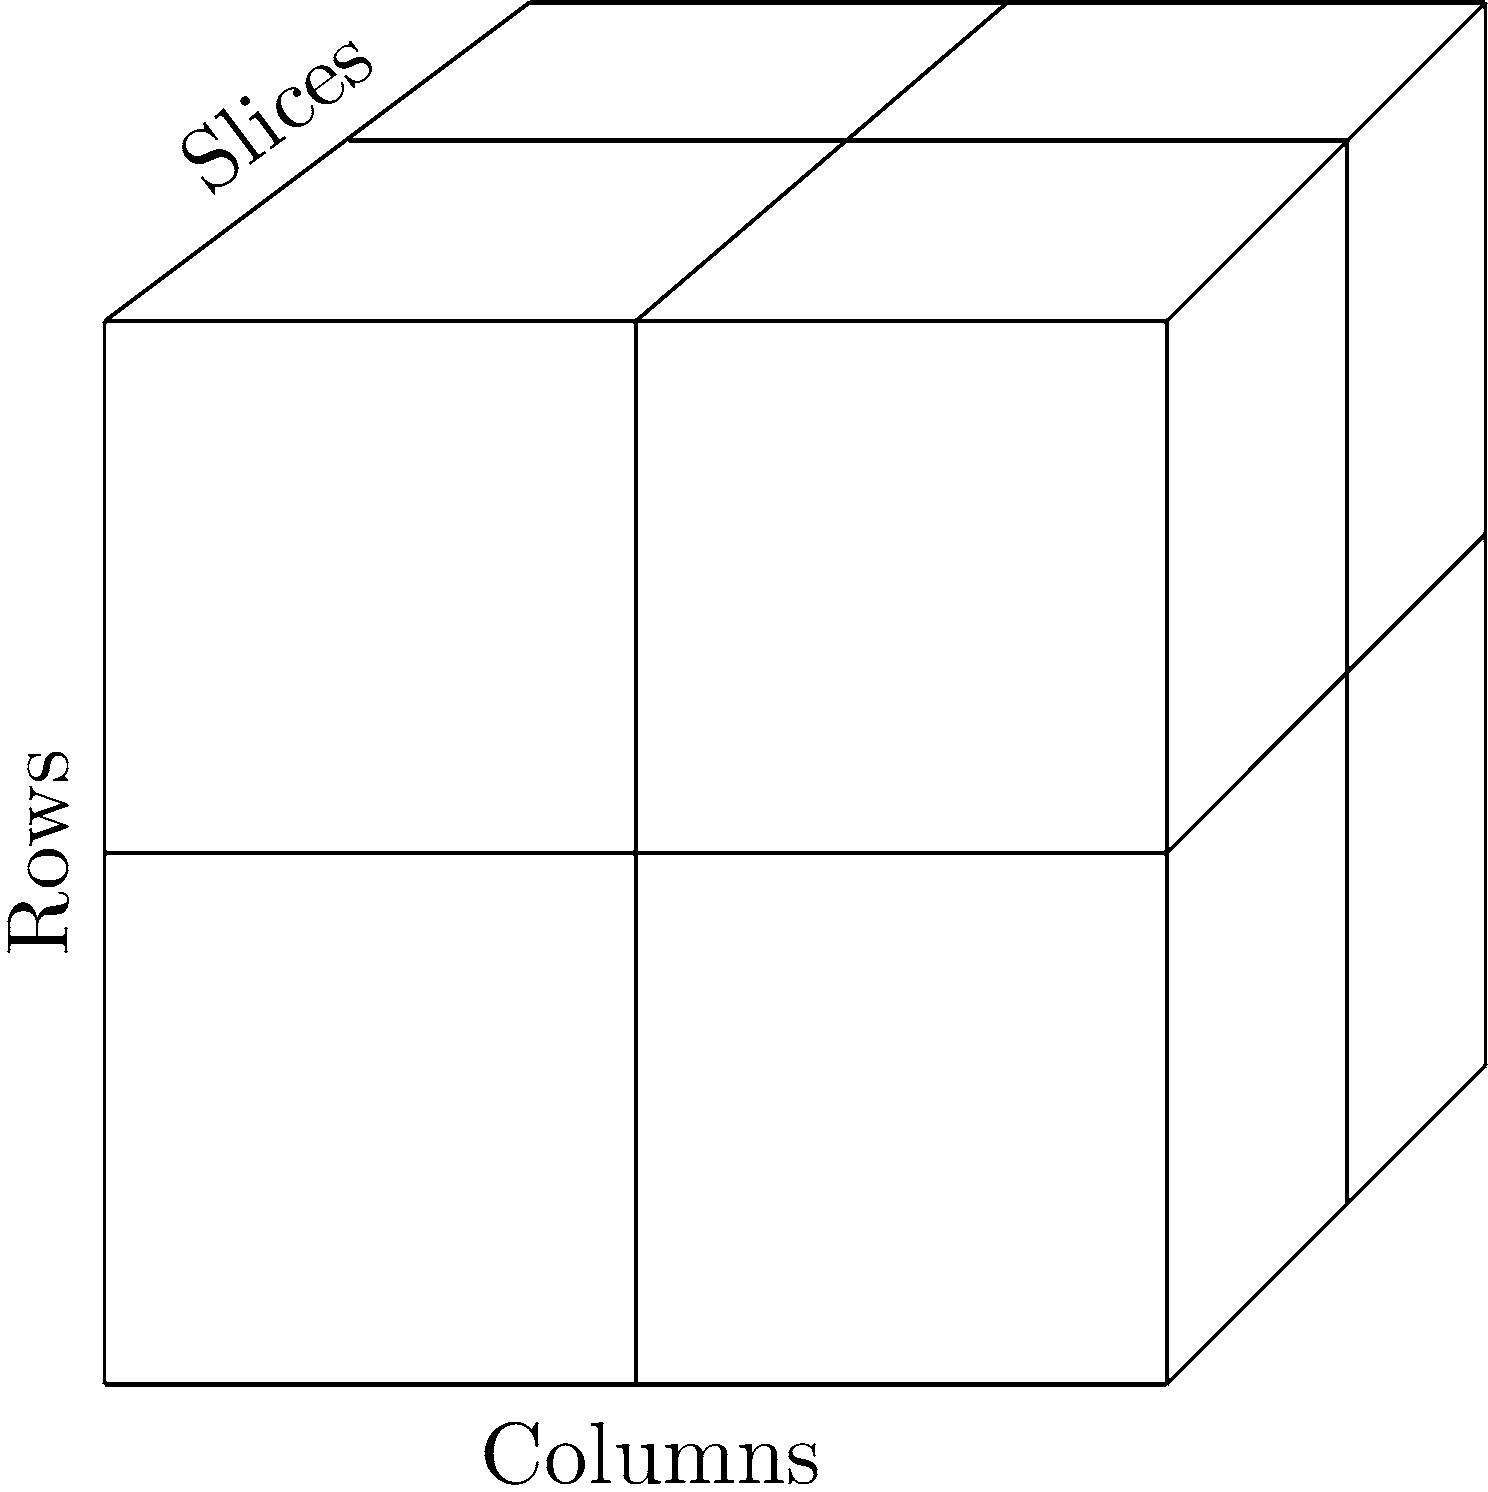
\includegraphics[width=5cm]{graficos/contingencia2x2x2} 

}

\caption{\label{fig:contingencia}Representación gráfica de una tabla de contingencia 2x2x2}\label{fig:unnamed-chunk-2}
\end{figure}

donde \(n_{ijk}\) denota la frecuencia de la celda de la i-ésima fila,
j-ésima columna y k-ésimo ¿corte? para \(i, j, k = 1, 2\). Sea
\(n_{i..}\) la frecuencia marginal de la i-ésima fila,
\(i = 1, . . . , r\); \(n_{.j.}\) la frecuencia marginal de la j-ésima
columna, \(j = 1, . . . ,c\), y \(n_{..k}\) la frecuencia marginal del
¿corte?-ésimo, \(k = 1, . . . s\). Por lo tanto, \(A = n_{1..}\),
\(B = n_{.1.}\), \(C = n_{..1}\), y \(N = n_{...}\) denotan los totales
de frecuencia marginal observados de la primera fila, la primera
columna, el primer ¿corte? y toda la tabla, respectivamente, de manera
que \(1 \le A \le B \le C \le N/2\). Además, sea \(w = n_{111}\),
\(x = n_{112}\), \(y = n_{121}\) y \(z = n_{211}\) las frecuencias de
las celdas de la tabla de contingencia \(2\times2\times2\). Entonces, la
probabilidad para cualquier \(w\), \(x\), \(y\), y \(z\) está dada por:

\[
P(w,x,y,z|A,B,C,N)=[A!(N-A)!B!(N-B)!C!(N-C)!]\times
\]

\[
\times[(N!)^2w!x!y!z!(A-w-x-y)!(B-w-x-z)!(C-w-y-z)!(N-A-B-C+2w+x+y+z)!]^{-1}
\]

\citep{Mielke1994}. Un algoritmo para calcular la probabilidad exacta de
Fisher implica una estructura de bucle anidado y requiere dos etapas. En
la primera se obtiene la probabilidad exacta, \(U\), de la tabla de
contingencia \(2\times2\times2\) observada. En la segunda etapa se
obtiene el valor de la probabilidad exacta de todas las tablas con
valores de probabilidad puntual hipergeométrica iguales o inferiores a
la probabilidad puntual de la tabla de contingencia observada. Los
cuatro bucles anidados dentro de cada etapa son sobre los índices de
frecuencia de las celdas \(w\), \(x\), \(y\) y \(z\), respectivamente.
Los límites de \(w\), \(x\), \(y\) y \(z\) son

\[
0\le w\le M_w,~~0\le x\le M_x,~~0\le y\le M_y~~~ y~~~ L_x\le z\le M_z,
\]

respectivamente, donde \(M_w = A\), \(M_x = A-w\), \(M_y = A-w-x\),
\(M_z = min(B -w- x,C - w - y)\), y
\(L_z = max(0,A + B + C - N - 2w - x - y)\).

El método de recursión puede ilustrarse con el cuarto bucle (interno)
sobre \(z\), dado \(w\), \(x\), \(y\), \(A\), \(B\), \(C\), y \(N\)
porque el bucle interno produce tanto \(U\) en la primera etapa como el
valor exacto de la probabilidad en la segunda etapa. Sea
\(H(w, x, y, z)\) una función recursiva positiva definida dados \(A\),
\(B\), \(C\) y \(N\), que satisface

\[
H(w,x,y,z+1)=H(w,x,y,z)\times g(w,x,y,z)~,
\]

donde

\[
g(w,x,y,z)=\frac{(B-w-x-z)(C-w-z)}{(z+1)(N-A-B-C+2w+x+y+z+1)}~.
\]

Los tres bucles restantes de cada etapa inicializan \(H(w, x, y, z)\).
Sea \(I_x = max(0,A + B + C - N)\) y se establece como valor inicial de
\(H(0, 0, 0, I_z)\) a una constante positiva arbitraria pequeña.
Entonces, el total sobre la distribución completamente enumerada sería:

\[
T=\sum_{w=0}^{M_w}\sum_{x=0}^{M_x}\sum_{y=0}^{M_y}\sum_{z=L_x}^{M_x}H(w,x,y,z)~.
\]

Si \(w_o\), \(x_o\), \(y_o\) y \(z_o\) son los valores de \(w\), \(x\),
\(y\) y \(z\) en la tabla de contingencia observada \(2\times2\times2\),
entonces \(U\) y el valor exacto de la probabilidad (\(P\)) vienen dados
por:

\[
U=H(w_o,x_o,y_o,z_o)/T
\]

y

\[
P=\sum_{w=0}^{M_w}\sum_{x=0}^{M_x}\sum_{y=0}^{M_y}\sum_{z=L_x}^{M_x}H(w,x,y,z)\psi(w,x,y,z)/T~,
\]

respectivamente, donde

\[
\psi(w,x,y,z)=\begin{cases}1 & si~~H(w,x,y,z)\le H(w_o,x_o,y_o,z_o) \\0 & si~~c.c.\end{cases} ~.
\]

\bibliography{bib/export.bib}


\addcontentsline{toc}{chapter}{Bibliografía}


\end{document}
